\documentclass[11pt,a4paper]{report}
\usepackage{graphicx,epsfig}
\usepackage{amsfonts}
\usepackage{amsthm, amsmath}
\usepackage{xcolor}
\usepackage{textcomp}
\usepackage{listings}
\usepackage[authoryear,round]{natbib}
\usepackage[hidelinks]{hyperref}
\usepackage{todonotes}
\usepackage{mathtools}
\usepackage{algorithm2e}
\usepackage{graphicx}
\usepackage{svg}
\usepackage{tabularx}

\usepackage{geometry}
\geometry{margin=2cm}

\newcommand*\diff{\mathop{}\!\mathrm{d}}
\DeclareMathOperator{\trace}{trace}
\DeclareMathOperator{\diag}{diag}
\DeclareMathOperator*{\argmax}{arg\,max}
\DeclareMathOperator*{\argmin}{arg\,min}

\newcolumntype{Y}{>{\centering\arraybackslash}X}

\graphicspath{ {./figures/} }

\parindent=25pt
\parskip 0.10in

\date{}
\begin{document}
\newgeometry{margin=4cm}

\thispagestyle{empty}
\begin{center}
{\huge
Gradient-Free Optimal Postprocessing \\
of MCMC Output

\bigskip
\bigskip

by
\bigskip
\bigskip

Artem Glebov
}
\end{center}
\vfill

\begin{center}
{\large
Department of Mathematics\\
King's College London\\
The Strand, London WC2R 2LS\\
United Kingdom\\
\medskip

}
\end{center}
\bigskip


\newpage
\setcounter{page}{1}
\restoregeometry

\chapter*{Abstract}


\tableofcontents


\chapter*{Introduction}

The Python code accompanying this report can be found at:
\begin{center}
\url{https://github.com/aglebov/gradient-free-mcmc-postprocessing}.
\end{center}

The implementation of the gradient-free kernel Stein thinning was contributed by the author directly to the \texttt{stein-thinning} Python library:
\begin{center}
\url{https://github.com/wilson-ye-chen/stein_thinning}.
\end{center}

\chapter{Background}

\section{Markov chain Monte Carlo (MCMC)}

Markov chain Monte Carlo (MCMC) are a popular class of algorithms for sampling from complex probability distributions.

The need to sample from a probability distribution arises in exploratory analysis as well as when analytical expressions are unavailable for quantities of interest, such as the modes or quantiles of the distribution, or for expectations with respect to the distribution, so a numerical simulation is used to obtain approximations instead. Such cases are frequent in Bayesian analysis, where the posterior density often has a complex structure with an analytically intractable normalising constant.

In the simplest cases where the inverse cumulative density function of a distribution is available, sampling can be done using the straightforward inverse method. Bespoke sampling methods, such as the Box-Muller transform for the normal distribution, can occasionally be developed by exploiting the properties of specific distributions. See Chapters 2 and 3 in \cite{robertMonteCarloStatistical2004} for an overview of these methods. Typically though, the complexity of the target distribution and the dimensionality of the parameter space render the simple methods infeasible or inefficient. Randomised algorithms, such as MCMC, have arisen to address the ensuing challenge.

\todo[inline]{Describe alternatives: the inverse method, accept-reject and importance sampling}

An MCMC algorithm proceeds by sequentially constructing a chain of samples\footnote{These are also sometimes called ``draws''. In this report, we follow the literature in using the term ``sample'' both for a single element in an MCMC chain and for all such elements taken together as a sample from the target distribution.} $x_1$, $x_2$, $\dots$,  where each sample is drawn from a transition distribution $Q$ conditional on the preceding value:
$$x_{n+1} \sim Q(x_{n+1}|x_n).$$
The distribution $Q$ is known as the transition kernel and is selected so that it is easy to sample from and to ensure asymptotic convergence to the target distribution $\Pi$:
$$x_n \xrightarrow[]{d} \Pi \quad\text{as}\quad n \to \infty.$$

Two classical variations of this technique are the Metropolis-Hastings and Gibbs algorithms.

\paragraph{Metropolis-Hastings algorithm.} The algorithm due to \cite{metropolisEquationStateCalculations1953} and \cite{hastingsMonteCarloSampling1970} uses an auxiliary distribution $q$ to sample a proposed value
$$x' \sim q(x' | x_n),$$
which is then accepted with probability
$$\alpha(x_n, x') = 1 \wedge \frac{\pi(x')}{\pi(x_n)} \frac{q(x_n|x')}{q(x'|x_n)}.$$
If $x'$ is accepted, the algorithm sets $x_{n+1} = x'$. If $x'$ is rejected, the value remains unchanged: $x_{n+1} = x_n$.

\todo[inline]{Consider using a different notation to avoid the confusion between the density of the proposal $q$ and the transition kernel $Q$.}

The common choice for the proposal distribution $q$ is a symmetric proposal satisfying $q(x'|x_n) = q(x_n|x')$, so that the ratio of these two quantities disappears from the expression for the acceptance probability:
$$\alpha(x_n, x') = 1 \wedge \frac{\pi(x')}{\pi(x_n)}.$$
In the special case where $q(x'|x_n) = q(x' - x_n)$ we obtain a random walk proposal:
$$x' = x_n + Z,$$
where $Z$ is the distribution of the step taken by the algorithm, e.g. a multivariate normal distribution. The operation of the algorithm then resembles a random walk across the domain of the target distribution where steps towards areas of lower probability are more likely to be rejected. The scale of the step distribution $Z$ determines the average size of the jump that the algorithm can make in one iteration and thus the speed of traversal of the target domain.

An alternative to symmetric proposals is an independence proposal satisfying $q(x'|x_n) = q(x')$.

\todo[inline]{Cite the ST03 lecture notes or Robert \& Casella}

\paragraph{Gibbs algorithm.} Suppose $x$ is a $d$-dimensional vector and the components $x^{(1)}$, $x^{(2)}$, $\dots$, $x^{(d)}$ can be partitioned in such a way that we can sample the components belonging to each partition while keeping the components in other partitions fixed. That is, let $I_i \subset \{1, \dots, d\}$ with $\cup_{i=1}^k I_i = \{1, \dots, d\}$ for some $k$ and $I_i \cap I_j = \emptyset$ for $i \neq j$, and assume we can sample
$$x^{(I_i)} \sim f_i\left(x^{(I_i)} | x^{(I_1, \dots, I_{i-1}, I_{i+1}, \dots, I_k)}\right).$$
The sample $x_{n+1}$ can then be constructed by sequentially sampling for each partition:
$$x_{n+1}^{(I_i)} \sim f_i\left(x^{(I_i)} | x_{n+1}^{(I_1, \dots, I_{i-1})}, x_n^{(I_{i+1}, \dots, I_k)}\right).$$
Note that the newly sampled values $x_{n+1}^{(I_1, \dots, I_{i-1})}$ enter the computation for subsequent partitions.

\todo[inline]{Read and cite the original paper for Gibbs sampler}

\todo[inline]{Consider simplifying this description}

\todo[inline]{Mention HMC and other recent variations}

Development of general-purpose and specialised MCMC algorithms remains an active area of research.

\section{Challenges of running MCMC}

While the asymptotic convergence of MCMC samples to the target distribution is guaranteed, no general guarantee is available for finite samples, resulting in several interrelated challenges that a practitioner faces when applying this class of algorithms:
\begin{enumerate}
\item The choice of a starting point for a chain affects the speed of convergence to the target distribution.
\item For a multimodal distribution, the algorithm might struggle to move between the modes within a feasible time. This problem becomes especially acute in high dimensions.
\item The scale of the proposal distribution must be calibrated to ensure that the algorithm is able to explore the domain of the target distribution efficiently.
\item Assessing how close an MCMC chain is to convergence is difficult, since the knowledge about the target distribution often comes from the chain itself.
\item In order to eliminate the impact of the starting point, it can be useful to discard the initial iterations of an MCMC chain, which are considered as ``burn-in''. Selecting the optimal length of the burn-in period is contingent on being able to detect convergence.
\item The sequential procedure of constructing a chain induces autocorrelation between the samples, which leads to increased variance of derived estimators.
\item The large number of samples resulting from an MCMC algorithm needs to be summarised for subsequent analysis, particularly when the cost of using all available samples is too high. Such situations arise when samples obtained from MCMC are used as starting points for further expensive simulations.
\end{enumerate}

The first three challenges require decisions to be made upfront before running the algorithm or adaptively during its run. In order to address the impact of the starting point, running multiple chains with starting points sampled from an overdispersed distribution is recommended~(\cite{gelmanInferenceIterativeSimulation1992}). This approach has the added benefit of increasing the chance of discovering the modes of the target distribution, although it does not provide a guarantee in this respect. 
\todo[inline]{Mention perfect sampling.}

Comparing the summary statistics of several chains (\cite{gelmanInferenceIterativeSimulation1992,brooksGeneralMethodsMonitoring1998,vehtariRankNormalizationFoldingLocalization2021}) offers a way to detect a lack of convergence at the cost of additional computation. Alternatively, the comparison can be applied to batches of samples from a single chain, as proposed by \cite{vatsRevisitingGelmanRubin2021}. Convergence detection can be used to terminate the algorithm once a chosen criterion is satisfied, or to assess the quality of a sample retrospectively. It should be noted that convergence criteria establish a necessary but not sufficient condition for convergence, so the outcomes need to be interpreted accordingly.

The scaling of the step distribution in a random-walk Metropolis-Hastings algorithm is commonly tuned to target the acceptance rate of roughly 0.234 for proposed samples (\cite{gelmanEfficientMetropolisJumping1996,gelmanWeakConvergenceOptimal1997,robertsOptimalScalingVarious2001}), which balances the speed of traversal and the computational effort generating samples that end up rejected.

The last three challenges are typically addressed by post-processing a sample from a completed MCMC run. A recent proposal by~\cite{riabizOptimalThinningMCMC2022} addresses these challenges by selecting a fixed-size subset of samples from an MCMC run such that the empirical distribution given by the subset best approximates the distribution resulting from the full sample. In the following section, we consider their approach in greater detail.

\todo[inline]{Read and cite Cowles and Carlin (1996) regarding the choice of burn-in length.}

\section{Optimal thinning}

Given a Markov chain $(X_i)_{i \in \mathbb{N}}$ and its realisation $(x_i)_{i=1}^n$ of length $n$, the empirical approximation of the target posterior distribution is given by
\begin{equation}
\frac{1}{n} \sum_{i=1}^n \delta(x_i),
\label{eq:discrete-distribution}
\end{equation}
where $\delta(x)$ is the Dirac delta function.
\cite{riabizOptimalThinningMCMC2022} set out to identify $m \ll n$ indices $\pi(j) \in \{1,\dots, n\}$ with $j\in\{1, \dots, m\}$, such that the approximation provided by the subset of samples
\begin{equation}
\frac{1}{m} \sum_{j=1}^m \delta(x_{\pi(j)})
\label{eq:thinned-sample}
\end{equation}
is closest to the approximation given by the full set, and thus to the target distribution. The criterion of proximity is based on the kernel Stein discrepancy, itself a special case of the integral probability metric.

\subsection{Kernel Stein discrepancy}

The integral probability metric between two distributions $P$ and $P'$ is defined as
\begin{equation}
\mathcal{D}_{\mathcal{F}}(P, P') \coloneq \sup_{f \in \mathcal{F}}\left|\int_\mathcal{X} f \diff P - \int_\mathcal{X} f \diff P' \right|,
\label{eq:ipm}
\end{equation}
where $\mathcal{X}$ is a measurable space on which both $P$ and $P'$ are defined and $\mathcal{F}$ is a set of test functions. Depending on the choice of $\mathcal{F}$, the definition~(\ref{eq:ipm}) gives rise to different classes of probability metrics, including the well-known Kolmogorov distance, Wasserstein distance and total variation distance.

If $P$ is taken to be the target distribution of an MCMC algorithm, evaluating~(\ref{eq:ipm}) poses two practical challenges:
\begin{itemize}
\item the integral $\int_\mathcal{X} f \diff P$ is often analytically intractable,
\item the supremum requires a non-trivial optimisation procedure to find.
\end{itemize}

The need to integrate with respect to $P$ can be eliminated if we find a set of function $\mathcal{F}$ for which $\int_\mathcal{X} f \diff P = 0$ for all $f \in \mathcal{F}$. The expression~(\ref{eq:ipm}) then simplifies to
\begin{equation}
\mathcal{D}_{\mathcal{F}}(P, P') = \sup_{f \in \mathcal{F}}\left|\int_\mathcal{X} f \diff P' \right|.
\label{eq:stein-discrepancy-sup}
\end{equation}

\cite{gorhamMeasuringSampleQuality2015} propose choosing such a set $\mathcal{F}$ based on the observation that the infinitesimal generator
$$(\mathcal{L}u)(x) = \lim_{t \to 0} \frac{\mathbb{E}[u(Z_t) | Z_0 = x] - u(x)}{t} \quad \text{for } u:\mathbb{R}^d \to \mathbb{R}$$
of a Markov process $(Z_t)_{t \geq 0}$ with stationary distribution $P$ satisfies 
$$\mathbb{E}[(\mathcal{L} u)(Z)] = 0$$
under mild conditions on $\mathcal{L}$ and $u$\todo[inline]{Check the conditions.}. In the specific case of an overdamped Langevin diffusion
$$\diff Z_t = \frac{1}{2} \nabla \log p(Z_t) \diff t + \diff W_t,$$
where $W_t$ is the standard Brownian motion, the infinitesimal generator becomes
$$(\mathcal{L}_P u)(x) = \frac{1}{2} \langle \nabla u(x), \nabla \log p(x)\rangle + \frac{1}{2}\langle \nabla, \nabla u(x) \rangle.$$
Denoting $g  = \frac{1}{2}\nabla u$, they obtain the Stein operator
\begin{equation}
\mathcal{A}_P g = \langle g, \nabla \log p \rangle + \langle \nabla, g \rangle = \langle p^{-1}\nabla, p g \rangle,
\label{eq:stein-operator}
\end{equation}
and rewrite~(\ref{eq:stein-discrepancy-sup}) as
\begin{equation}
\mathcal{D}_{P, \mathcal{G}}(P') = \sup_{g \in \mathcal{G}}\left|\int_\mathcal{X} \mathcal{A}_P g \diff P' \right|
\label{eq:stein-discrepancy-g}
\end{equation}
for a suitably chosen set $\mathcal{G}$. Note that $p$ enters~(\ref{eq:stein-operator}) via $\nabla \log p$, so the knowledge of its normalising constant is not required to evaluate the operator.

To remove the optimisation step in the calculation of~(\ref{eq:stein-discrepancy-g}), \cite{gorhamMeasuringSampleQuality2017} employ a reproducing kernel Hilbert space (RKHS) $\mathcal{H}(k)$ with kernel $k: \mathbb{R}^d \times \mathbb{R}^d \to \mathbb{R}$ satisfying the reproducing property:
$$f(x) = \langle f, k(x, \cdot)\rangle \quad\text{for } f \in \mathcal{H}(k).$$
Taking the set
\begin{equation}
\mathcal{G} \coloneq \left\{ \mathrm{g} : \mathbb{R}^d \to \mathbb{R}^d \left| \sum_{i=1}^d \|g_i\|^2_{\mathcal{H}(k)} \leq 1 \right.\right\}
\label{eq:unit-ball}
\end{equation}
which defines a unit-ball in a Cartesian product of $d$ copies $\mathcal{H}(k)$, Proposition~2 in \cite{gorhamMeasuringSampleQuality2017} establishes that
\begin{equation}
\mathcal{D}_{P}^2(P') = \mathbb{E}_{P' \times P'}[k_P(X, \tilde{X})] = \iint_\mathcal{X} k_P(x, y) \diff p'(x) \diff p'(y),
\label{eq:stein-discrepancy-sqrt-expectation}
\end{equation}
where $X, \tilde{X} \sim P'$, $p'$ is the density of $P'$, and $k_P(x, y)$ is given by
\begin{equation}
\begin{aligned}
k_P(x, y) \coloneq 
&(\nabla_x\cdot\nabla_y) k(x,y) \\
&+ \langle \nabla_x k(x, y), \nabla_y \log p(y) \rangle + \langle \nabla_y k(x, y), \nabla_x \log p(x) \rangle \\
&+ k(x, y) \langle \nabla_x \log p(x), \nabla_y \log p(y) \rangle.
\label{eq:deriv:stein-kernel}
\end{aligned}
\end{equation}
Here $\nabla_x$ and $\nabla_y$ are gradients w.r.t.\ $x$ and $y$, respectively, and the operator $\nabla_x\cdot\nabla_y$ is defined as:
$$(\nabla_x\cdot\nabla_y) k(x,y) \coloneq \sum_{i=1}^d \frac{\partial^2}{\partial x_i\, \partial y_i} k(x, y).$$
Note that we have dropped $\mathcal{G}$ in the subscript of~(\ref{eq:stein-discrepancy-sqrt-expectation}) as the choice of $\mathcal{G}$ does not depend on $P$ or $P'$.
If $P'$ is a discrete distribution, as in~(\ref{eq:discrete-distribution}), the squared discrepancy~(\ref{eq:stein-discrepancy-sqrt-expectation}) becomes
\begin{equation}
\mathcal{D}_{P}^2\left(\frac{1}{n} \sum_{i=1}^n \delta(x_i)\right) = \frac{1}{n^2} \sum_{i,j=1}^n k_P(x_i, x_j).
\label{eq:ksd:discrete}
\end{equation}

When $k(x, y)$ is chosen to be the inverse multiquadratic kernel (IMQ)
\begin{equation}
k(x, y) = \left(c^2 + \|\Gamma^{-1/2}(x-y)\|\right)^\beta
\label{eq:imq}
\end{equation}
with $\beta \in (-1, 0)$, \cite{gorhamMeasuringSampleQuality2017} demonstrate for $\Gamma = I$ that $\mathcal{D}_{P}(P')$ provides convergence control:
\begin{itemize}
\item if $\mathcal{D}_{P}(P'_m) \to 0$, then $P'_m$ converges in distribution to $P$ (Theorem 8),
\item if $P'_m$ converges to $P$ in Wasserstein distance, then $\mathcal{D}_{P}(P'_m) \to 0$ (Proposition 9)
\end{itemize}
for a sequence of distributions $P'_m$ under suitable conditions. Theorem 4 by \cite{chenSteinPointMarkov2019} justifies the introduction of $\Gamma$ in IMQ.

The constant $c$ in~(\ref{eq:imq}) can be set to 1 without loss of generality, and the positive-definite preconditioner matrix $\Gamma$ can be chosen to exploit the geometry of the parameter space. \cite{riabizOptimalThinningMCMC2022} suggest several choices for $\Gamma$, in particular the identity matrix scaled by the median Euclidean distance between points in the sample, possibly further rescaled by $(\log m)^{-1/2}$ where $m$ is the desired cardinality of the thinned sample, or the sample covariance matrix. Based on empirical evaluation, \cite{gorhamMeasuringSampleQuality2017} and \cite{riabizOptimalThinningMCMC2022} settle on the value $\beta = -\frac12$.

The expression for $k_P(x, y)$ when $k(x, y)$ is taken to be the inverse multiquadratic kernel is derived in section~\ref{appendix:derivations:imq-stein} and is coded directly in the Python library \texttt{stein-thinning}\footnote{Available from \url{https://github.com/wilson-ye-chen/stein_thinning}.}.

Other choices of kernels are possible and offer convergence control, as demonstrated by \cite{chenSteinPoints2018}, however IMQ performed on par or better than the alternatives considered by the authors.

\subsection{Stein thinning}
\label{sec:stein-thinning}

Equipped with the kernel Stein discrepancy (KSD) as defined above, \cite{riabizOptimalThinningMCMC2022} develop a greedy optimisation algorithm to select a subset of points from a sample that minimises the total kernel Stein discrepancy. Rather than attempting to evaluate KSD for all $n \choose m$ combinations of points, they construct a subsample iteratively, each time picking a point that minimises the KSD with previously selected points. We reproduce their procedure verbatim in Algorithm~\ref{alg:cap} for the reader's convenience. 

\begin{algorithm}
\caption{Stein thinning.}\label{alg:cap}
\KwData{Sample $(x_i)_{i=1}^n$ from MCMC, Stein kernel $k_P$, desired cardinality $m \in \mathbb{N}$.}
\KwResult{Indices $\pi$ of a sequence $(x_{\pi(j)})_{j=1}^m \subset \{x_i\}_{i=1}^n$ where $\pi(j) \in \{1, \dots, n\}$.}

\For{$j = 1, \dots, m$}{
$$\pi(j) \in \argmin_{i=1,\dots,n} \frac{k_P(x_i, x_i)}{2} + \sum_{j'=1}^{j-1} k_P(x_{\pi(j'}, x_i)$$
}
\end{algorithm}

The algorithm was implemented by the authors and made available in the open-source library \texttt{stein-thinning}. The computational complexity of the provided implementation is $O(nm)$.

The strength of the method lies in its ability to correct for bias in the input sample, as established by Theorem 3 in \cite{riabizOptimalThinningMCMC2022}, meaning that the algorithm can be applied to samples from MCMC chains that have not converged to the target distribution, provided that its domain is sufficiently explored by the chains. The limitation of the method comes from its reliance on the gradients of the log-target, which may be expensive to compute.

\subsection{Gradient-free kernel Stein discrepancy}

\todo[inline]{Cite cases where gradient cannot be computed easily.}

To address the limitation of the kernel Stein discrepancy, \cite{fisherGradientFreeKernelStein2024} propose the gradient-free Stein operator $\mathcal{S}_{P,Q}$ defined for any differentiable function $g$ as
\begin{equation}
\mathcal{S}_{P,Q} g \coloneq \frac{q}{p}(\langle g, \nabla \log q \rangle + \langle \nabla, g \rangle) = \frac{q}{p} \langle q^{-1}\nabla, q g \rangle.
\end{equation}
This definition generalises expression~(\ref{eq:stein-operator}) by introducing a proxy distribution $Q$ with density $q$ chosen such that its gradient is easily computable. When $q = p$, we recover the original Langevin Stein operator~(\ref{eq:stein-operator}).

\cite{fisherGradientFreeKernelStein2024} proceed to show in their Proposition 1 that, under certain regularity conditions,
\begin{equation*}
\int_\mathcal{X} \mathcal{S}_{P,Q} g \diff P = 0
\end{equation*}
for any function $g$ whose first derivatives exist and are bounded, allowing them to define the gradient-free kernel Stein discrepancy
\begin{equation*}
\mathcal{D}_{P, Q}(P') = \sup_{g \in \mathcal{G}}\left|\int_\mathcal{X} \mathcal{S}_{P,Q} g \diff P' \right|
\end{equation*}
by analogy with~(\ref{eq:stein-discrepancy-g}), taking $\mathcal{G}$ again to be the unit-ball~(\ref{eq:unit-ball}). Futhermore, Proposition 7 in \cite{fisherGradientFreeKernelStein2024} establishes that
\begin{equation*}
\mathcal{D}_{P, Q}^2(P') = \iint_\mathcal{X} \frac{q(x)}{p(x)} \frac{q(y)}{p(y)} k_Q(x, y) \diff p'(x) \diff p'(y),
\label{eq:gf-ksd:int}
\end{equation*}
where $p'$ is the density of distribution $P'$ and $k_Q(x, y)$ is given by~(\ref{eq:deriv:stein-kernel}) but with $q$ replacing $p$. For a discrete $P'$, this translates to
\begin{equation}
\mathcal{D}_{P, Q}^2\left(\frac{1}{n} \sum_{i=1}^n \delta(x_i)\right) = \frac{1}{n^2} \sum_{i,j=1}^n \frac{q(x_i)}{p(x_i)} \frac{q(x_j)}{p(x_j)} k_Q(x_i, x_j).
\label{eq:gf-ksd:discrete}
\end{equation}

Both expression~(\ref{eq:ksd:discrete}) and~(\ref{eq:gf-ksd:discrete}) can be viewed as averaging the elements of matrices, and this fact is used to provide an efficient implementation of the greedy search described in Section~\ref{sec:stein-thinning}.

When $k_Q(x,y)$ is based on IMQ with $\Gamma = I$, Theorem 2 in \cite{fisherGradientFreeKernelStein2024} proves that $\mathcal{D}_{P, Q}^2(P_m') \to 0$ implies that the sequence of distributions $P'_m$ converges weakly to $P$ as $m \to \infty$, thus ensuring convergence control. 

While removing the need to calculate the gradient of log-target, the approach by \cite{fisherGradientFreeKernelStein2024} replaces it with the requirement to choose a suitable proxy distribution $Q$. The authors provide several examples:
\begin{itemize}
\item where the target distribution is the posterior in a Bayesian inference problem, the prior distribution can serve as $Q$,
\item where $p$ can be differentiated, the Laplace approximation of $P$ could be used,
\item where samples from $P$ are available, it can be approximated by either the Gaussian mixture model (GMM) or a kernel density estimator (KDE).
\end{itemize}

The choice of a proxy is non-trivial, and \cite{fisherGradientFreeKernelStein2024} warn of possible failure of convergence control when the proxy density $q$ has either a substantially heavier or a substantially lighter tail than $p$. Two other situations are identified by the authors as detrimental to their approach: high dimension of the domain $\mathcal{X}$ and well separated high-probability regions.

In their paper, \cite{fisherGradientFreeKernelStein2024} apply gradient-free KSD for importance resampling and variational inference problems. In this dissertation, we adopt their approach for the thinning problem.

\chapter{Methodology and Results}

We modify Algorithm~\ref{alg:cap} to use the gradient-free Stein kernel $k_{P,Q}(x,y)$ in place of $k_P(x, y)$. With the inverse multiquadratic kernel~(\ref{eq:imq}), this results in the expression
\begin{equation*}
\begin{aligned}
k_{P,Q}(x, y)
= &\frac{q(x)}{p(x)} \frac{q(y)}{p(y)} \times \\
 &\left[ -4 \frac{\beta(\beta-1) \| \Gamma^{-1}(x - y)\|^2}{(c^2 + \| \Gamma^{-1/2}(x-y)\|^2)^{-\beta-2}} \right.  \\
&- 2 \beta \frac{\trace(\Gamma^{-1}) + \langle \Gamma^{-1} (x - y), \nabla_x \log q(x) - \nabla_y \log q(y)\rangle}{(c^2 + \| \Gamma^{-1/2}(x-y)\|^2)^{-\beta-1}} \\
& \left. + \frac{\langle \nabla_x \log q(x), \nabla_y \log q(y) \rangle}{(c^2 + \| \Gamma^{-1/2}(x-y)\|^2)^{-\beta}} \right]. \\
\end{aligned}
\label{eq:k_Q}
\end{equation*}

The implementation is added directly to the publicly available Python library \texttt{stein-thinning}.

We proceed to compare the performance of the proposed algorithm against na\"ive thinning (retaining each $i$-th element of the sample) and the Stein thinning algorithm of \cite{riabizOptimalThinningMCMC2022} for several target distributions. The outline of the evaluation procedure for each test case is as follows:
\begin{enumerate}
\item obtain a sample from the target distribution,
\item apply na\"ive thinning, Stein thinning and the proposed algorithm to get a thinned sample of a given cardinality,
\item calculate the energy distance between the thinned sample and the target distribution and compare the values across the algorithms.
\end{enumerate}

In order to assess how well the selected sample approximates the posterior distribution, we use the energy distance. Following \cite{rizzoEnergyDistance2016}, the squared energy distance is defined for two distributions $F$ and $G$ as
$$D^2(F, G) \coloneq 2 \mathbb{E} \|X - Y\| - \mathbb{E}\|X - X'\| - \mathbb{E} \|Y - Y'\|,$$
where $X, X' \sim F$, $Y, Y' \sim G$, and $\|\cdot\|$ denotes the Euclidean norm. For samples $x_1, \dots, x_n$ and $y_1, \dots, y_m$ from $X$ and $Y$, respectively, the corresponding statistic is given by
\begin{equation*}
\mathcal{E}_{n,m}(X, Y) \coloneq \frac{2}{nm}\sum_{i=1}^n \sum_{j=1}^m \|x_i - y_j\| - \frac{1}{n^2} \sum_{i=1}^n\sum_{j=1}^n \|x_i - x_j\| - \frac{1}{m^2} \sum_{i=1}^m \sum_{j=1}^m \|y_i - y_j\|.
\label{eq:energy-distance:discrete}
\end{equation*}

The advantages of choosing the energy distance as our quality metric are its relative ease of computation and its objectivity, since the energy distance is not directly optimised by the thinning algorithm.

We use synthetic data in order to have control over the ground truth in our experiments.

\section{Bivariate Gaussian mixture}
\label{sec:gaussian-mixture}

The purpose of the first test case is to confirm the expected behaviour of the proposed algorithm under favourable conditions. Here we take the target distribution to be the bivariate Gaussian mixture with means 
$$
\mu_1 = \begin{pmatrix} -1 \\ -1 \end{pmatrix}, \qquad
\mu_2 = \begin{pmatrix} 1 \\ 1 \end{pmatrix},
$$
covariance matrices
$$
\Sigma_1 = \begin{pmatrix}
0.5 & 0.25\\
0.25 & 1
\end{pmatrix}, \qquad
\Sigma_2 = \begin{pmatrix}
2 & -0.8 \sqrt{3}\\
-0.8 \sqrt{3} & 1.5
\end{pmatrix}
$$
and weights
$$w = \begin{pmatrix} 0.3 \\ 0.7 \end{pmatrix},$$
and obtain 1000 samples by directly drawing from the target. A scatter plot of the sample as well as the contour plot of the probability density are shown in Figure~\ref{fig:gmm:sample}.

\begin{figure}[h]
\centering
\makebox[\textwidth][c]{
	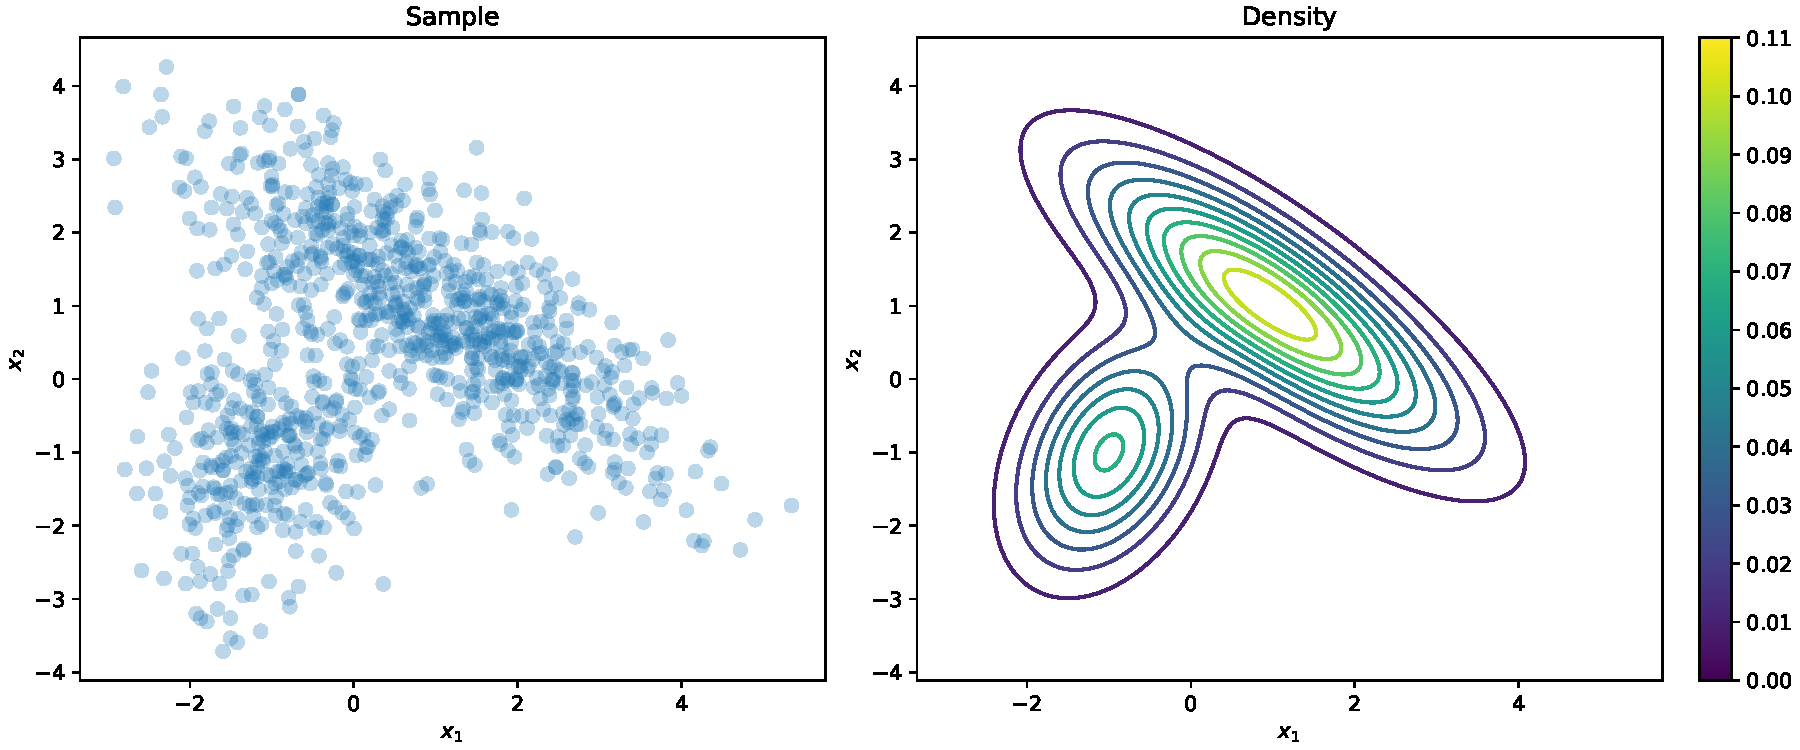
\includegraphics[width=1.0\textwidth]{gaussian-mixture-sample.pdf}
}
\caption{A sample from the bivariate Gaussian mixture with two components and its probability density function.
\label{fig:gmm:sample}}
\end{figure}

\paragraph{Na\"ive thinning.} We select elements of the sample with uniformly-spaced indices.

\paragraph{Stein thinning.} The gradients of the log-target required by the Stein thinning algorithm can be obtained analytically in this case. For multivariate normal distributions with density functions
$$f_i(\mathbf{x}) = \frac{1}{(2\pi)^{d/2} |\Sigma_i|^{1/2}}\exp\left(-\frac{1}{2}(\mathbf{x} - \pmb{\mu}_i)^T \Sigma_i^{-1}(\mathbf{x}-\pmb{\mu}_i)\right),$$
where $\mathbf{x} \in \mathbb{R}^d$, the mixture density with $k$ components is given by
$$f(\mathbf{x}) = \sum_{i=1}^k w_i f_i(\mathbf{x}),$$
thus the gradient of the log-density is obtained as
$$\nabla_{\mathbf{x}} \log f(\mathbf{x}) = \frac{\sum_{i=1}^k w_i \nabla_{\mathbf{x}} f_i(\mathbf{x})}{\sum_{i=1}^k w_i f_i(\mathbf{x})} = -\frac{\sum_{i=1}^k w_i f_i(\mathbf{x}) \Sigma_i^{-1}(\mathbf{x} - \pmb{\mu}_i)}{\sum_{i=1}^k w_i f_i(\mathbf{x})}.$$

\paragraph{Gradient-free Stein thinning.} This approach requires us to select a proxy distribution. We consider several options:
\begin{itemize}
\item a bivariate Gaussian with the mean and covariance matrix matching the sample mean and covariance of the sample,
\item a Laplace approximation of the target distribution,
\item a KDE approximation of the target constructed from the sample.
\end{itemize}

For the KDE estimator, we choose the Gaussian kernel with bandwidth selected according to Silverman's rule.

The results are shown in Figure~\ref{fig:gmm:thinned}. The failure of the Laplace proxy is striking, so we investigate it further. The other methods produce visually sensible results. One can notice some clustering of points selected by na\"ive thinning, whereas the Stein thinning and the gradient-free approach using the Gaussian proxy and the KDE proxy appear to spread points more evenly.

\begin{figure}[h]
\centering
\makebox[\textwidth][c]{
	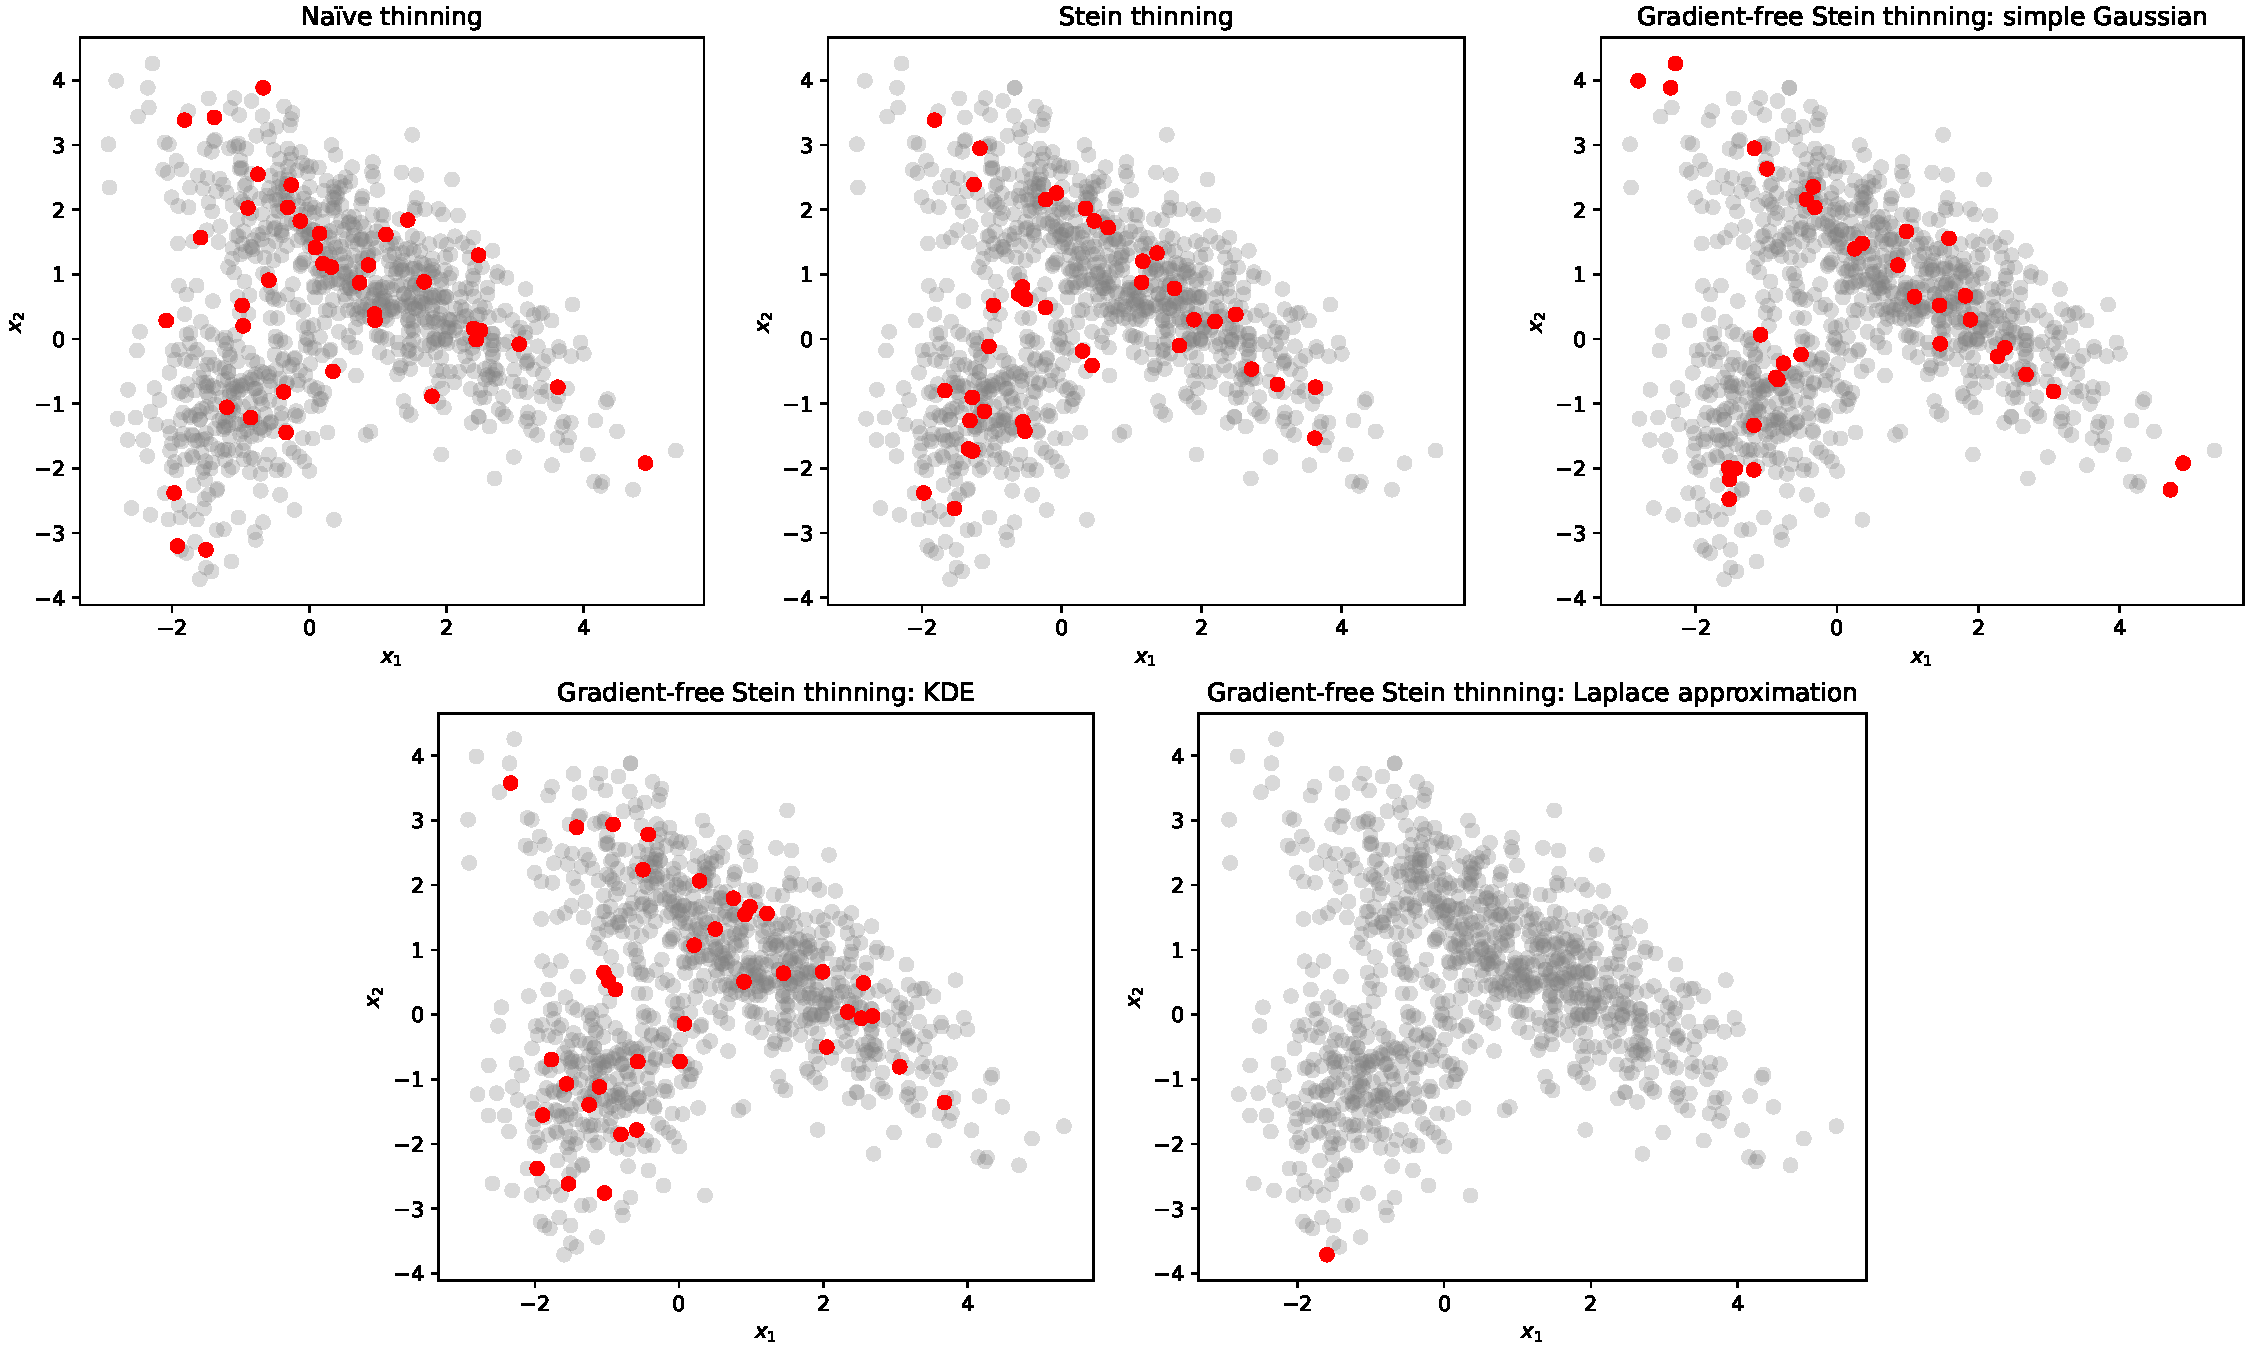
\includegraphics[width=1.0\textwidth]{gaussian-mixture-thinned-20.pdf}
}
\caption{Thinning results for the bivariate Gaussian mixture.
\label{fig:gmm:thinned}}
\end{figure}

To see why the Laplace approximation fails in this case, note the multiplier $q(x) / p(x)$ in~(\ref{eq:gf-ksd:discrete}). Since the thinning algorithm seeks to minimise the sum, it will tend to prefer elements with low values of $q(x) / p(x)$. In Figure~\ref{fig:gmm:laplace-failure}, we plot the values $\log q(x) - \log p(x) = \log (q(x) / p(x))$ for points in the sample. It is clear that the points in the lower left corner of the plot become very attractive for the algorithm to select due to their miniscule values of the multiplier $q(x) / p(x)$. The low ratio $q(x) / p(x)$ for those points is in turn due to the fact that the Laplace approximation picks the larger of the two modes in the mixture, so it cannot serve as a good proxy for the samples coming from the other component. By contract, the simple Gaussian proxy achieves more uniform values of the multiplier.

\begin{figure}[h]
\centering
\makebox[\textwidth][c]{
	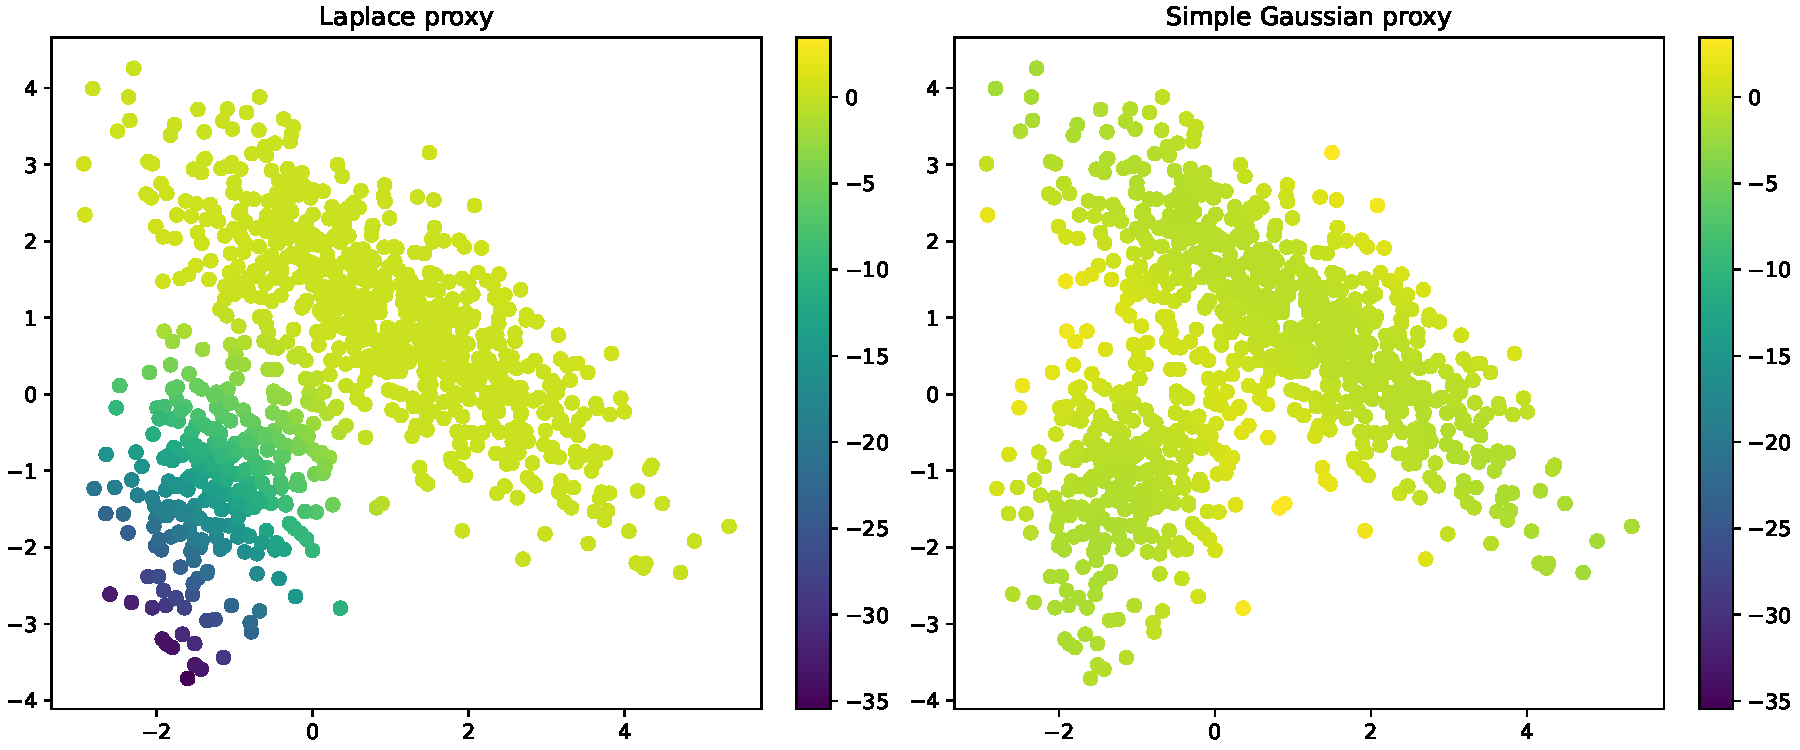
\includegraphics[width=1.0\textwidth]{gaussian-mixture-laplace-proxy.pdf}
}
\caption{The values of $\log q(x) - \log p(x)$ for the points in the Gaussian mixture sample under the Laplace proxy and the simple Gaussian proxy using the sample mean and covariance.
\label{fig:gmm:laplace-failure}}
\end{figure}

Finally, Figure~\ref{fig:gmm:comparison} compares the energy distance achieved by thinned samples using the approaches above. We see that the gradient-free approach using the KDE proxy is competitive with Stein thinning for small cardinalities, but loses out as the required sample size grows. The gradient-free approach using the simple Gaussian proxy proves inferior to the na\"ive approach.

\begin{figure}[h]
\centering
\makebox[\textwidth][c]{
	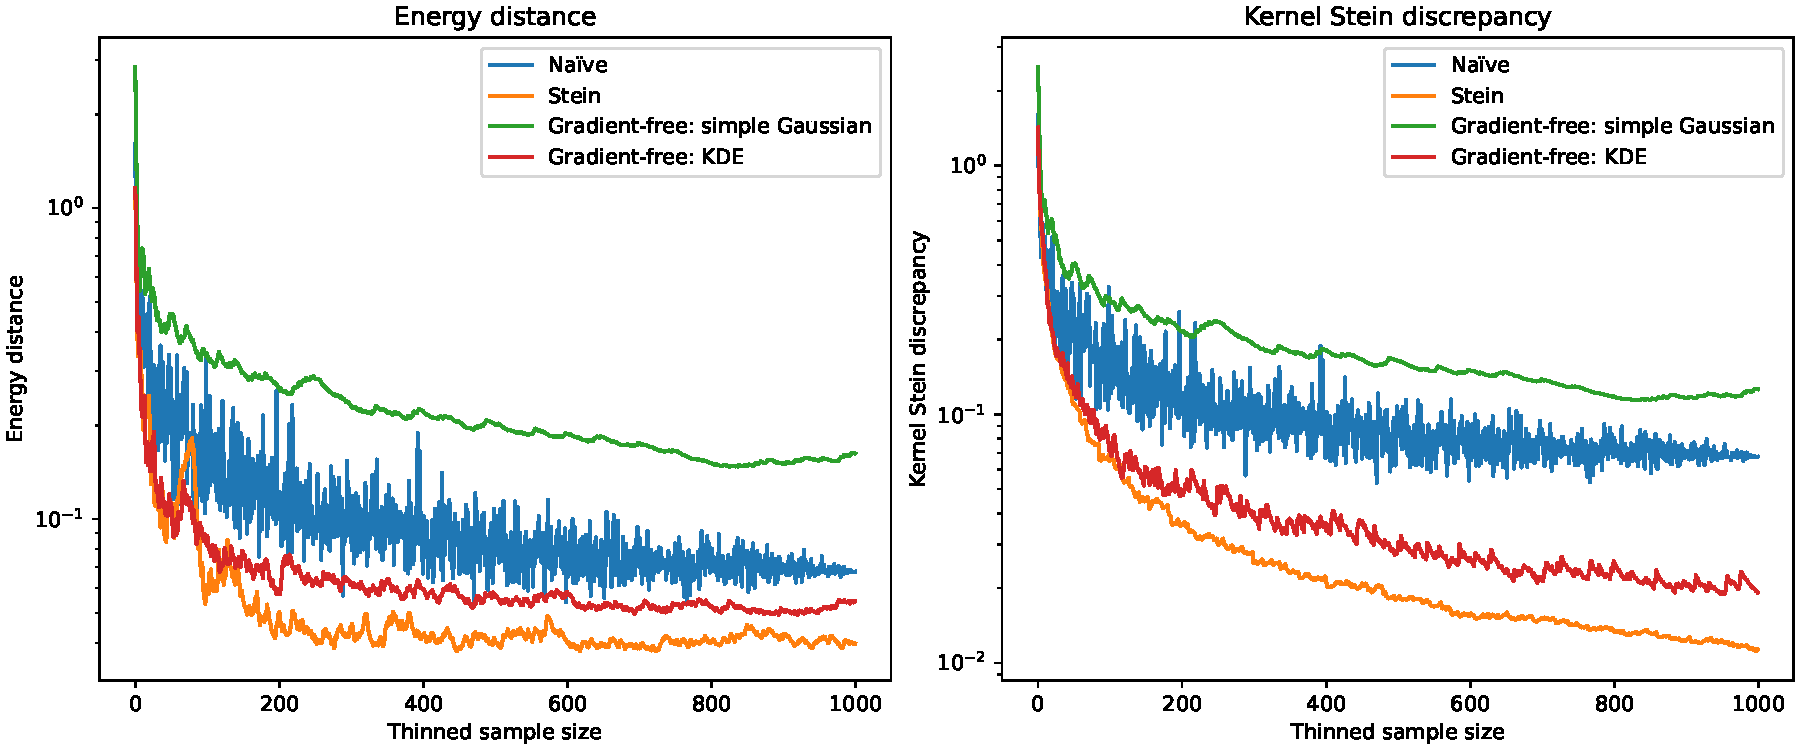
\includegraphics[width=0.6\textwidth]{gaussian-mixture-comparison.pdf}
}
\caption{Energy distance comparison between thinning approaches for the bivariate Gaussian mixture sample.
\label{fig:gmm:comparison}}
\end{figure}

We conclude that even in such a favourable setup, the performance of the gradient-free algorithm depends crucially on the choice of the proxy distribution.

\section{Lotka-Volterra inverse problem}
\label{sec:lotka-volterra}

A more challenging case is presented by the inverse problem of parameter inference for the Lotka-Volterra model.

\todo[inline]{Cite sources on inverse Bayesian problems.}

The Lotka-Volterra model describes the evolution of an idealised ecosystem with two species: predator and prey. The predator population grows when prey is abundant, and the prey population shrinks when there are too many predators. Denoting the size of prey population by $u_1$, and the predator population by $u_2$, the model postulates the following dynamic:
%\begin{equation}
%\begin{alignat*}{4}
%\frac{\diff u_1}{u_1} & = ( &  \theta_1 & & - \theta_2 u_2 & ) & & \diff t \\
%\frac{\diff u_2}{u_2} & = ( & -\theta_3 & & + \theta_4 u_1 & ) & & \diff t \\
%\end{alignat*}
%\end{equation}
\begin{equation}
\begin{aligned}
\frac{\diff u_1}{u_1} & = ( \;\;\;\theta_1 - \theta_2 u_2 ) \diff t \\
\frac{\diff u_2}{u_2} & = ( -\theta_3 + \theta_4 u_1 ) \diff t \\
\end{aligned}
\label{eq:lotka-volterra}
\end{equation}
The resulting behaviour is driven by the four parameters $\theta_1, \dots, \theta_4$. It is convenient to denote the solution to this system as  $\mathbf{u}(t;\pmb{\theta}) = (u_1(t; \pmb{\theta}), u_2(t; \pmb{\theta}))^T$, where $\pmb{\theta}$ is the vector of parameter values $(\theta_1, \dots, \theta_4)^T$.

If a realisation of $\mathbf{u}(t; \pmb{\theta})$ is observed for an interval $t \in [0, T]$ with $\pmb{\theta}$ unknown, one may wish to infer the values of the parameters that best describe the observed behaviour. In a practical setting, this corresponds to formulating a parametric model for a natural phenomenon and inferring the parameters of the model from the measurements of the phenomenon. We emulate this situation by fixing the true model, generating a realisation perturbed by noise and then attempting to recover the parameters of the true model from the realisation.

We take $\mathbf{u}(t;\pmb{\theta}^*)$ to be generated for $t \in [0, 25]$ by the model~(\ref{eq:lotka-volterra}) with parameters $\pmb{\theta}^* = (0.67, 1.33, 1, 1)^T$ and initial value $\mathbf{u}(0; \pmb{\theta}^*) = (1, 1)^T$. The interval $[0, 25]$ is discretised into $N = 2400$ points, so that $t_i = 25 \cdot i / N$ for $i \in \{0, 2400\}$. Bivariate i.i.d.\ Gaussian noise $\pmb{\varepsilon}(t) \sim \mathcal{N}\left( \mathbf{0}, \diag(0.2^2, 0.2^2) \right)$ is then added to all data points to emulate the measurement error, and we take the resulting time series $\mathbf{y}(t) = \mathbf{u}(t;\pmb{\theta}^*) + \pmb{\varepsilon}(t)$ as our observed data. Figure~\ref{fig:lotka-volterra:data} displays the values $\mathbf{y}(t)$. For comparability of results, the parameter values above match those used by \cite{riabizOptimalThinningMCMC2022}. 

\begin{figure}[h]
\centering
\makebox[\textwidth][c]{
	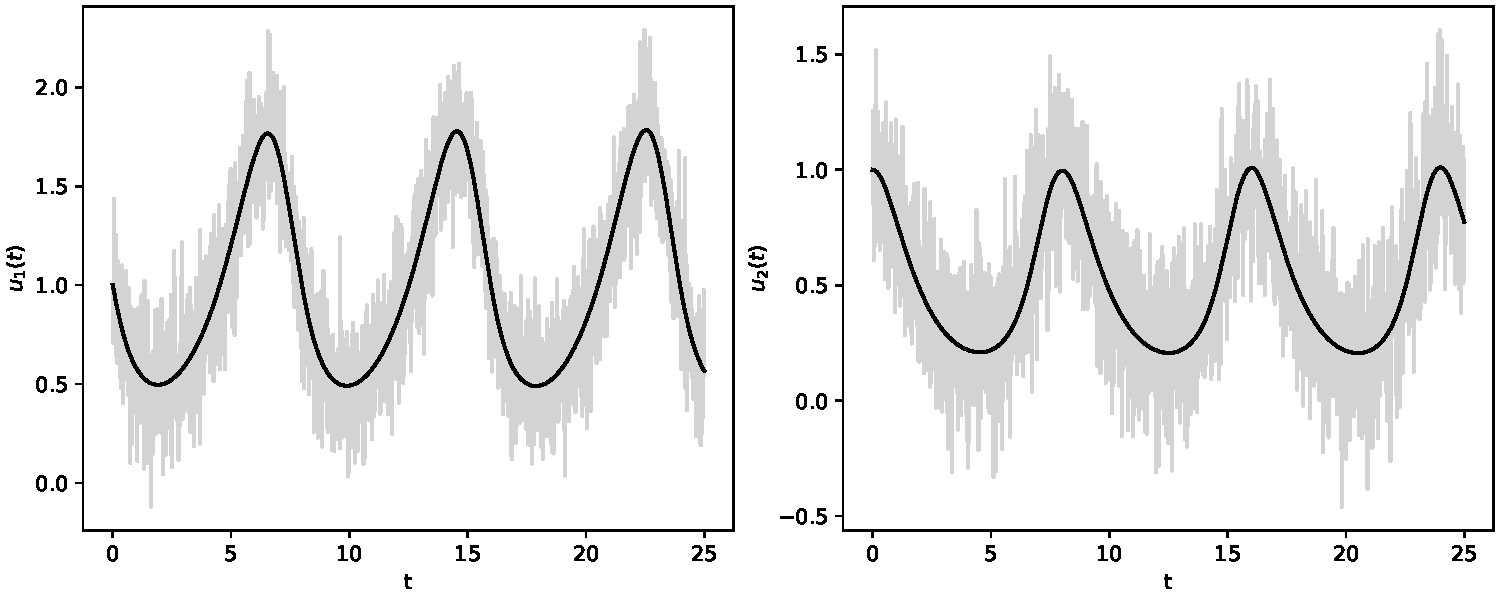
\includegraphics[width=1.0\textwidth]{lotka-volterra.pdf}
}
\caption{Solution to the Lotka-Volterra ODEs (black) with added Gaussian noise (grey).
\label{fig:lotka-volterra:data}}
\end{figure}

Inference is then performed by means of a random-walk Metropolis-Hastings algorithm. Note that the likelihood is not available in an explicit form in this case, but is instead determined by the deviation of the solution $\mathbf{u}(t;\pmb{\theta})$ from $\mathbf{y}(t)$ for each $\pmb{\theta}$. Specifically, we take
\begin{equation}
\mathcal{L}(\pmb{\theta}) = \prod_{i=1}^N \phi_i(\mathbf{u}(t_i; \pmb{\theta})),
\label{eq:lotka-volterra:likelihood}
\end{equation}
where 
\begin{equation}
\phi_i(\mathbf{u}(t_i;\pmb{\theta})) \propto \exp\left( -\frac{1}{2} (\mathbf{y}(t_i) - \mathbf{u}(t_i; \pmb{\theta}))^T C^{-1} (\mathbf{y}(t_i) - \mathbf{u}(t_i; \pmb{\theta})) \right)
\label{eq:lotka-volterra:error-distr}
\end{equation}
with $C = \diag(0.2^2, 0.2^2)$. We also put independent standard normal priors on each of $\log \theta_i$, so that
\begin{equation}
\pi(\pmb{\theta}) \propto \exp \left(-\frac{1}{2} (\log \pmb{\theta})^T (\log \pmb{\theta}) \right),
\label{eq:lotka-volterra:prior}
\end{equation}
where the logarithm in $\log \pmb{\theta}$ is applied component-wise.
By the Bayes theorem, the posterior is then
\begin{equation}
p(\pmb{\theta}) \propto \mathcal{L}(\pmb{\theta}) \pi(\pmb{\theta}).
\label{eq:lotka-volterra:posterior}
\end{equation}
We follow \cite{riabizOptimalThinningMCMC2022} in selecting the starting values for the chains (Table~\ref{table:lotka-volterra:starting_values}).

\begin{table}[h!]
\centering
\begin{tabularx}{0.5\textwidth}{c Y Y Y Y} 
 \hline
 Chain & $\theta_1$ & $\theta_2$ & $\theta_3$ & $\theta_4$ \\
 \hline
 1 & 0.55 & 1    & 0.8 & 0.8 \\ 
 2 & 1.5  & 1    & 0.8 & 0.8 \\
 3 & 1.3  & 1.33 & 0.5 & 0.8 \\
 4 & 0.55 & 3    & 3.  & 0.8 \\
 5 & 0.55 & 1    & 1.5 & 1.5 \\
 \hline
\end{tabularx}
\caption{Starting values for the random-walk Metropolis-Hastings algorithm in the Lotka-Volterra inference problem.}
\label{table:lotka-volterra:starting_values}
\end{table}

Since the parameters of the Lotka-Volterra model are non-negative, we run inference in the log-space. The trace plots from running 500,000 iterations of the random-walk Metropolis-Hastings algorithm for each chain are shown in Figure~\ref{fig:lotka-volterra:trace-plots}. Figure~\ref{fig:lotka-volterra:chain-paths} confirms that all chains reach the high-probability region, albeit after considerable burn-in. Having obtained samples from the posterior distribution, we proceed to thin them.

\todo[inline]{Add example sample, e.g. from the first chain.}

\begin{figure}[h]
\centering
\makebox[\textwidth][c]{
	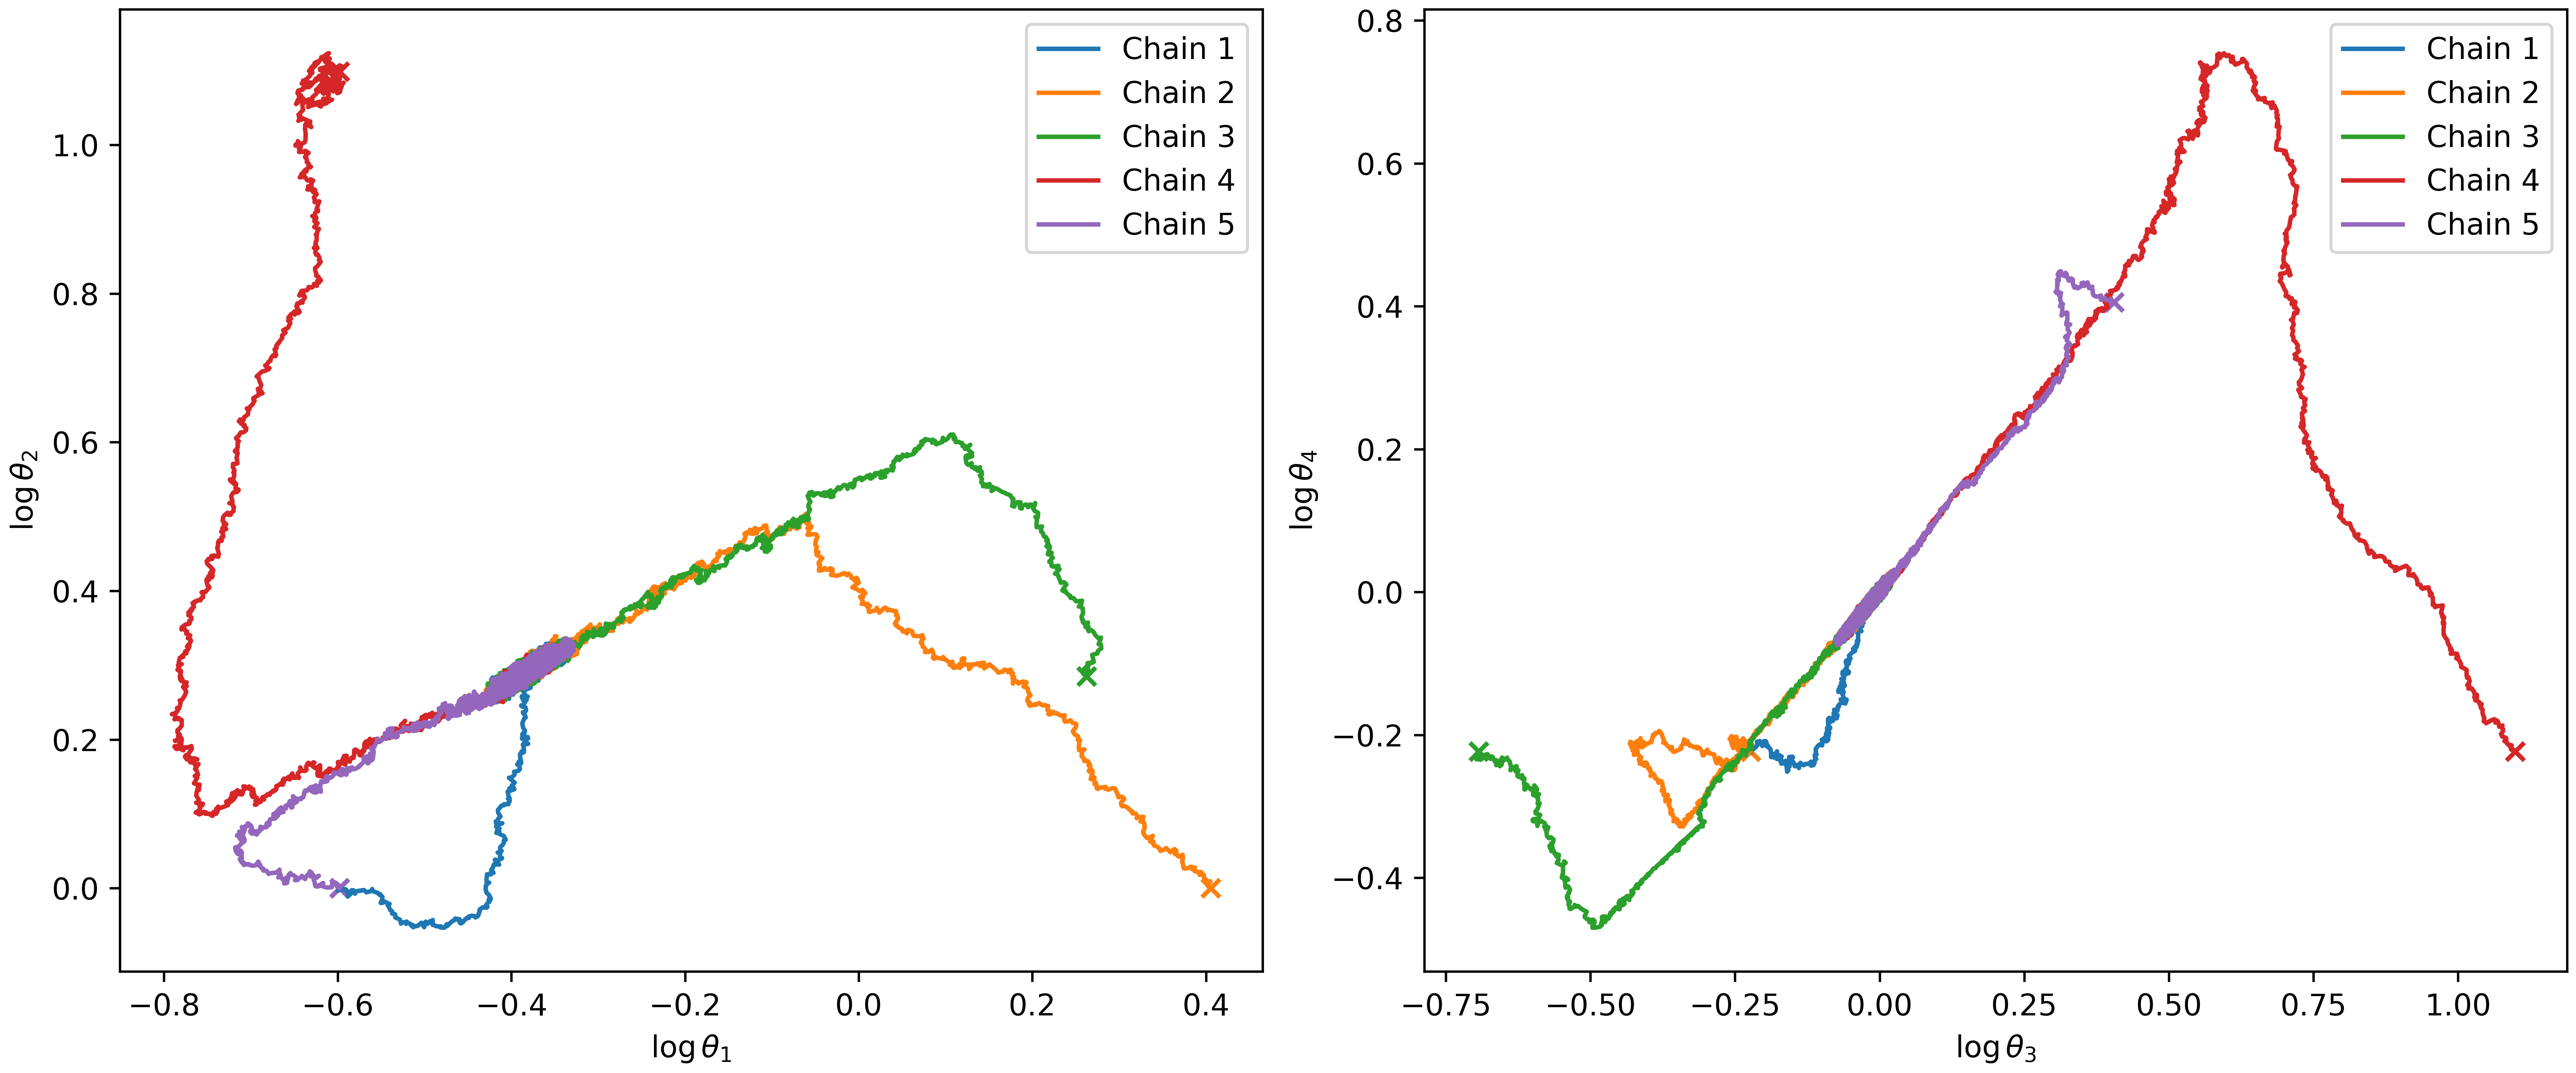
\includegraphics[width=1.0\textwidth]{lotka-volterra-chain-paths.png}
}
\caption{Chain paths from the random-walk Metropolis-Hastings algorithm for the Lotka-Volterra inference problem.
\label{fig:lotka-volterra:chain-paths}}
\end{figure}

\paragraph{Na\"ive thinning.} We select elements of the sample with uniformly spaced indices. The results are shown in Figure~\ref{fig:lotka-volterra:naive:results} in the Appendix.

\paragraph{Stein thinning.} In order to use this approach, we need the gradients of the log-posterior. From~(\ref{eq:lotka-volterra:posterior}), we have
\begin{equation*}
\nabla_{\pmb{\theta}} \log p(\pmb{\theta}) = \nabla_{\pmb{\theta}} \log \mathcal{L}(\pmb{\theta}) + \nabla_{\pmb{\theta}} \pi(\pmb{\theta}).
\end{equation*}
Equation~(\ref{eq:lotka-volterra:likelihood}) yields
\begin{equation*}
\frac{\partial}{\partial \theta_s} \log \mathcal{L}(\pmb{\theta}) 
= \sum_{i=1}^N \frac{\partial}{\partial \theta_s} \log \phi_i(\mathbf{u}(t_i; \pmb{\theta}))
= \sum_{i=1}^N \sum_{r=1}^q \frac{\partial}{\partial u_r} (\log \phi_i) \frac{\partial u_r}{\partial \theta_s},
\end{equation*}
where $q = 2$ is the dimension of the vector $\mathbf{u}(t)$ and $s \in \{1, \dots, 4\}$. This can be written in the matrix form as
\begin{equation*}
(\nabla_{\pmb{\theta}} \log \mathcal{L})(\pmb{\theta}) = \sum_{i=1}^N (S(t_i))^T (\nabla_{\mathbf{u}} \log \phi_i)(\mathbf{u}(t_i; \pmb{\theta})),
\end{equation*}
where the elements of the sensitivities matrix are given by
\begin{equation*}
S_{r,s} \coloneq \frac{\partial u_r}{\partial \theta_s}.
\end{equation*}
The gradient
\begin{equation*}
(\nabla_\mathbf{u} \log \phi_i)(\mathbf{u}(t_i; \pmb{\theta})) = C^{-1}(\mathbf{y}(t_i) - \mathbf{u}(t_i; \pmb{\theta}))
\end{equation*}
is derived directly from~(\ref{eq:lotka-volterra:error-distr}). In order to obtain the sensitivities $\frac{\partial u_r}{\partial \theta_s}$, we augment the system~(\ref{eq:lotka-volterra}) with additional forward sensitivity equations and solve it numerically. The derivation of the sensitivity equations can be found in Appendix~\ref{appendix:derivations:forward-sensitivity}. Alternatively, the sensitivities can be obtained by numerical differentiation, for example using the Python library \texttt{JAX}\footnote{\url{https://jax.readthedocs.io}}. Since the gradient is calculated independently for each element of the sample, these calculations can easily be parallelised\footnote{Parallelisation can be implemented with minimal effort using the Python \texttt{Dask} library (\url{https://docs.dask.org}) and run either locally or on Amazon Web Services (\url{https://aws.amazon.com}). See \url{https://github.com/aglebov/gradient-free-mcmc-postprocessing/blob/main/code/examples/Dask_AWS.ipynb} for a demonstration.}.

The gradient of the log-prior is obtained immediately from~(\ref{eq:lotka-volterra:prior}):
\begin{equation*}
\nabla_{\pmb{\theta}} \log \pi(\pmb{\theta}) = -\frac{\log \pmb{\theta}}{\pmb{\theta}},
\end{equation*}
where the logarithm and division are component-wise.

The results of applying Stein thinning are shown in Figure~\ref{fig:lotka-volterra:stein:results} in the Appendix. We compare the performance of Stein thinning in linear and log space of parameters in Figure~\ref{fig:lotka-volterra:stein-thinning:energy-distance}:
\begin{itemize}
\item there is no discernible difference between the linear and logarithmic parameterisations,
\item Stein thinning performs consistently for all chains, whereas na\"ive thinning fails for chain 4, which spent most of its time away from the high-probability region,
\item Stein thinning improves on na\"ive thinning for sample sizes below 20 and above 2000, and is otherwise similar.
\end{itemize}

\begin{figure}[h]
\centering
\makebox[\textwidth][c]{
	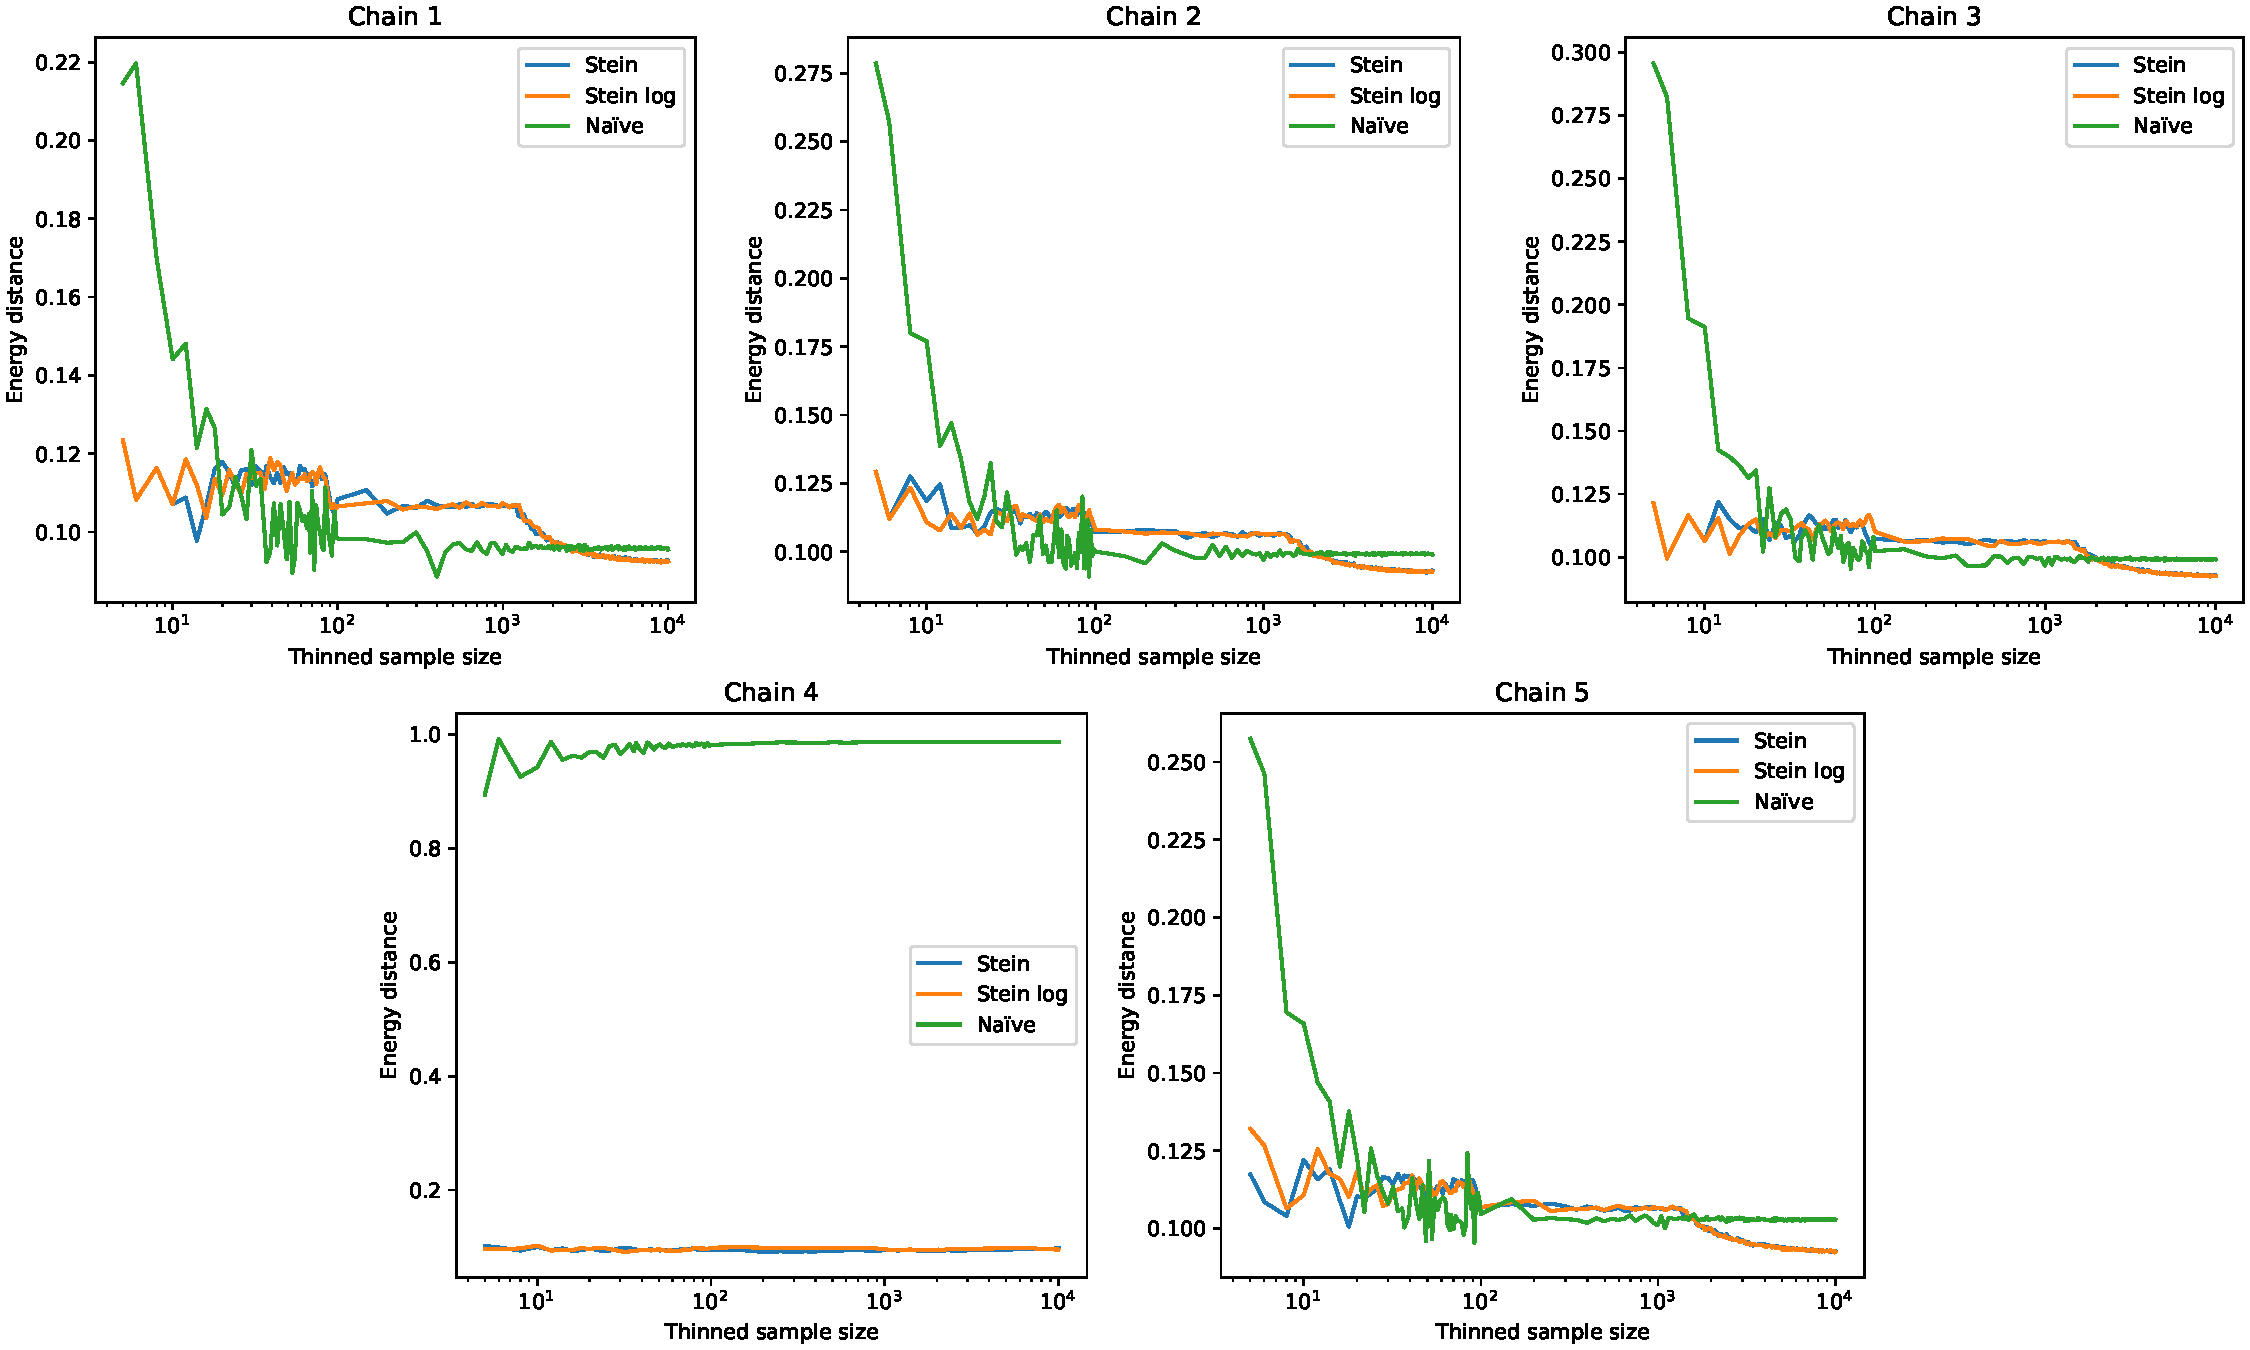
\includegraphics[width=1.0\textwidth]{lotka-volterra-stein-thinning-energy-distance.pdf}
}
\caption{Energy distance comparison between Stein thinning and na\"ive thinning for MCMC chains in the Lotka-Volterra inverse problem.
\label{fig:lotka-volterra:stein-thinning:energy-distance}}
\end{figure}

\paragraph{Gradient-free Stein thinning.} The KDE proxy, which performed best for the Gaussian mixture in Section~\ref{sec:gaussian-mixture}, becomes computationally infeasible here due to the size of the sample. Indeed, if KDE is built based on the entire sample, and is evaluated for each point of the sample, the resulting computational cost grows as $O(n^2)$, where $n$ is the sample size. One could try to build a KDE based on a subsample of size $m < n$, however if the computational budget is fixed (i.e. $mn = \text{const}$) then larger $n$ implies lower $m$ and thus inferior approximation of the target density.


\chapter{Conclusions and Further Work}
\label{sec:conclusions}

This dissertation offers two contributions:
\begin{itemize}
\item Implementation of the gradient-free thinning made available in the Python library \texttt{stein-thinning}.
\item Evaluation of the performance of the proposed approach for a Gaussian mixture and the Lotka-Volterra inverse problem.
\end{itemize}

We conclude that the gradient-free approach is feasible and performs similarly to the Stein thinning algorithm of \cite{riabizOptimalThinningMCMC2022} for small thinned sample sizes, however its performance depends crucially on the choice of the proxy distribution. Even in the highly favourable setting of a Gaussian mixture, choosing the proxy based on the Laplace approximation fails to produce a thinned sample, while a simple Gaussian proxy using the sample mean and covariance proves to be inferior to the na\"ive thinning approach. Bespoke treatment is required for more complex problems, as demonstrated by the case of parameter inference in the Lotka-Volterra model. In deciding whether to use the new algorithm as opposed to the gradient-based approach, the effort involved in selecting a good proxy must be weighed against the computational time that would otherwise be required to obtain gradients.

Many interesting avenues for further research remain open:
\begin{itemize}
\item Evaluate the choices of KDE kernels other than Gaussian for constructing the proxy distribution. Kernels with bounded support (uniform, saw-tooth, Epanechnikov) are expected to be of limited use, since they do not provide gradient estimates outside of their support, however fat-tailed kernels (e.g. exponential or Student's $t$) are an interesting option to consider.
\item Parallelise the computation of KDE. As noted in Section~\ref{sec:lotka-volterra}, the computational cost of the KDE approach rises as $O(n^2)$, where $n$ is the size of the sample. Evaluations of the density, however, can be performed in parallel, extending the range of sample sizes that can be handled within a given time budget.
\item Perform thinning in a lower-dimensional space. Samples from the MCMC runs for the Lotka-Volterra problem indicate correlation between the parameters. \todo{Refer to a figure showing the correlation between variables.} Principal component analysis (PCA) could be used to identify a lower-dimensional representation of the samples, and thinning could be done in the transformed space.
\end{itemize}

\bibliographystyle{plainnat_modified}
\bibliography{biblio}

\appendix
\chapter{Derivations}
\label{appendix:derivations}

\section{Stein kernel based on inverse multiquadratic kernel}
\label{appendix:derivations:imq-stein}

Given a kernel $k(x,y)$, the corresponding Stein kernel is given by~(\ref{eq:deriv:stein-kernel}). For the inverse multiquadratic kernel~(\ref{eq:imq}) we obtain
\begin{equation}
\begin{aligned}
\frac{\partial}{\partial x_r} k(x,y) 
%&= \beta \left(c^2 + \sum_{i=1}^d\sum_{j=1}^d (x_i-y_i) \Gamma^{-1}_{ij}(x_j-y_j)\right)^{\beta-1} \\
%&\times \left( \sum_{j=1}^d \Gamma^{-1}_{lj}(x_j - y_j) + \sum_{i=1}^d (x_i - x_j) \Gamma^{-1}_{il} \right) \\
&= \beta \left(c^2 + \sum_{i=1}^d\sum_{j=1}^d (x_i-y_i) \Gamma^{-1}_{ij}(x_j-y_j)\right)^{\beta-1}
\sum_{j=1}^d (\Gamma^{-1} + \Gamma^{-T})_{rj}(x_j - y_j) \\
&= 2 \beta \left(c^2 + \sum_{i=1}^d\sum_{j=1}^d (x_i-y_i) \Gamma^{-1}_{ij}(x_j-y_j)\right)^{\beta-1}
\sum_{j=1}^d \Gamma^{-1}_{rj}(x_j - y_j), \\
\end{aligned}
\end{equation}
where we used that $\Gamma$ is a symmetric matrix. The gradient is then
\begin{equation}
\nabla_x k(x,y) = 2 \beta \left(c^2 + \| \Gamma^{-1/2} (x-y)\|^2\right)^{\beta-1} \Gamma^{-1} (x - y).
\label{eq:appx:deviv:nablax}
\end{equation}
and similarly
\begin{equation}
\nabla_y k(x,y) = -2 \beta \left(c^2 + \| \Gamma^{-1/2} (x-y)\|^2\right)^{\beta-1} \Gamma^{-1} (x - y).
\label{eq:appx:deviv:nablay}
\end{equation}
Now
\begin{equation}
\begin{aligned}
\frac{\partial^2}{\partial x_r\,\partial y_r} k(x,y) 
= &-4 \beta(\beta-1) \left(c^2 + \sum_{i=1}^d\sum_{j=1}^d (x_i-y_i) \Gamma^{-1}_{ij}(x_j-y_j)\right)^{\beta-2} \left(\sum_{j=1}^d \Gamma^{-1}_{rj}(x_j - y_j)\right)^2 \\
&- 2\beta \left(c^2 + \sum_{i=1}^d\sum_{j=1}^d (x_i-y_i) \Gamma^{-1}_{ij}(x_j-y_j)\right)^{\beta-1} \Gamma^{-1}_{rr}
\end{aligned}
\end{equation}
which gives us
\begin{equation}
\begin{aligned}
(\nabla_x \cdot \nabla_y) k(x,y) 
&= -4 \beta(\beta-1) \left(c^2 + \| \Gamma^{-1/2}(x-y)\|^2\right)^{\beta-2} \| \Gamma^{-1}(x - y)\|^2 \\
&- 2\beta \left(c^2 + \|\Gamma^{-1/2}(x-y)\|^2\right)^{\beta-1} \trace(\Gamma^{-1})
\label{eq:appx:deriv:nablax_nablay}
\end{aligned}
\end{equation}

Substituting (\ref{eq:appx:deviv:nablax}), (\ref{eq:appx:deviv:nablay}) and (\ref{eq:appx:deriv:nablax_nablay}) into (\ref{eq:deriv:stein-kernel}), we obtain
\begin{equation}
\begin{aligned}
k_P(x, y)
= &-4 \beta(\beta-1) \left(c^2 + \| \Gamma^{-1/2}(x-y)\|^2\right)^{\beta-2} \| \Gamma^{-1}(x - y)\|^2 \\
&- 2\beta \left(c^2 + \|\Gamma^{-1/2}(x-y)\|^2\right)^{\beta-1} \trace(\Gamma^{-1}) \\
&+ 2 \beta \left(c^2 + \| \Gamma^{-1/2} (x-y)\|^2\right)^{\beta-1} \langle \Gamma^{-1} (x - y), \nabla_y \log p(y)\rangle \\
&- 2 \beta \left(c^2 + \| \Gamma^{-1/2} (x-y)\|^2\right)^{\beta-1} \langle \Gamma^{-1} (x - y), \nabla_x \log p(x)\rangle \\
&+ \left(c^2 + \| \Gamma^{-1/2} (x-y)\|^2\right)^\beta \langle \nabla_x \log p(x), \nabla_y \log p(y) \rangle \\
= &-4 \beta(\beta-1) D^{\beta-2} \| \Gamma^{-1}(x - y)\|^2  \\
&- 2 \beta D^{\beta-1} (\trace(\Gamma^{-1}) + \langle \Gamma^{-1} (x - y), \nabla_x \log p(x) - \nabla_y \log p(y)\rangle) \\
&+ D^\beta \langle \nabla_x \log p(x), \nabla_y \log p(y) \rangle, \\
\end{aligned}
\label{eq:k_P:IMQ}
\end{equation}
where we have denoted $D = c^2 + \| \Gamma^{-1/2}(x-y)\|^2$.

\section{Forward sensitivity equations for the Lotka-Volterra model}
\label{appendix:derivations:forward-sensitivity}

Given a system of ODEs of the form:
$$\frac{\diff u_r}{\diff t} = F_r(t, u_1, \dots, u_q; \theta_1, \dots, \theta_d),\qquad r=1,\dots,q,$$
where $q$ is the dimension of the state space (i.e.\ the number of observed variables) and $d$ is the dimension of the parameter space,
the sensitivities can be found by solving forward sensitivity equations:
$$\frac{\diff}{\diff t}\left(\frac{\partial u_r}{\partial \theta_s}\right)
= \frac{\partial}{\partial \theta_s}\frac{\diff u_r}{\diff t} 
%= \frac{\diff F_r}{\diff \theta_s} 
= \frac{\partial F_r}{\partial \theta_s} + \sum_{l=1}^q \frac{\partial F_r}{\partial u_l} \frac{\partial u_l}{\partial \theta_s}.$$

\todo[inline]{Double-check the notation above.}

For the Lotka-Volterra model~(\ref{eq:lotka-volterra}), this yields eight additional equations:
\begin{equation*}
\begin{aligned}
\frac{\diff}{\diff t}\left(\frac{\partial u_1}{\partial \theta_1}\right) &= u_1 + (\theta_1 - \theta_2 u_2) \frac{\partial u_1}{\partial \theta_1} - \theta_2 u_1 \frac{\partial u_2}{\partial \theta_1}, \\
\frac{\diff}{\diff t}\left(\frac{\partial u_1}{\partial \theta_2}\right) &= - u_1 u_2 + (\theta_1 - \theta_2 u_2) \frac{\partial u_1}{\partial \theta_2} - \theta_2 u_1 \frac{\partial u_2}{\partial \theta_2}, \\
\frac{\diff}{\diff t}\left(\frac{\partial u_1}{\partial \theta_3}\right) &= (\theta_1 - \theta_2 u_2) \frac{\partial u_1}{\partial \theta_3} - \theta_2 u_1 \frac{\partial u_2}{\partial \theta_3}, \\
\frac{\diff}{\diff t}\left(\frac{\partial u_1}{\partial \theta_4}\right) &= (\theta_1 - \theta_2 u_2) \frac{\partial u_1}{\partial \theta_4} - \theta_2 u_1 \frac{\partial u_2}{\partial \theta_4}, \\
\frac{\diff}{\diff t}\left(\frac{\partial u_2}{\partial \theta_1}\right) &= \theta_4 u_2 \frac{\partial u_1}{\partial \theta_1} + (\theta_4 u_1 - \theta_3) \frac{\partial u_2}{\partial \theta_1}, \\
\frac{\diff}{\diff t}\left(\frac{\partial u_2}{\partial \theta_2}\right) &= \theta_4 u_2 \frac{\partial u_1}{\partial \theta_2} + (\theta_4 u_1 - \theta_3) \frac{\partial u_2}{\partial \theta_2}, \\
\frac{\diff}{\diff t}\left(\frac{\partial u_2}{\partial \theta_3}\right) &= -u_2 + \theta_4 u_2 \frac{\partial u_1}{\partial \theta_3} + (\theta_4 u_1 - \theta_3) \frac{\partial u_2}{\partial \theta_3}, \\
\frac{\diff}{\diff t}\left(\frac{\partial u_2}{\partial \theta_4}\right) &= u_1 u_2 + \theta_4 u_2 \frac{\partial u_1}{\partial \theta_4} + (\theta_4 u_1 - \theta_3) \frac{\partial u_2}{\partial \theta_4}. \\
\end{aligned}
\end{equation*}

\chapter{Additional figures}
\label{appendix:figures}

\begin{figure}[h]
\centering
\makebox[\textwidth][c]{
	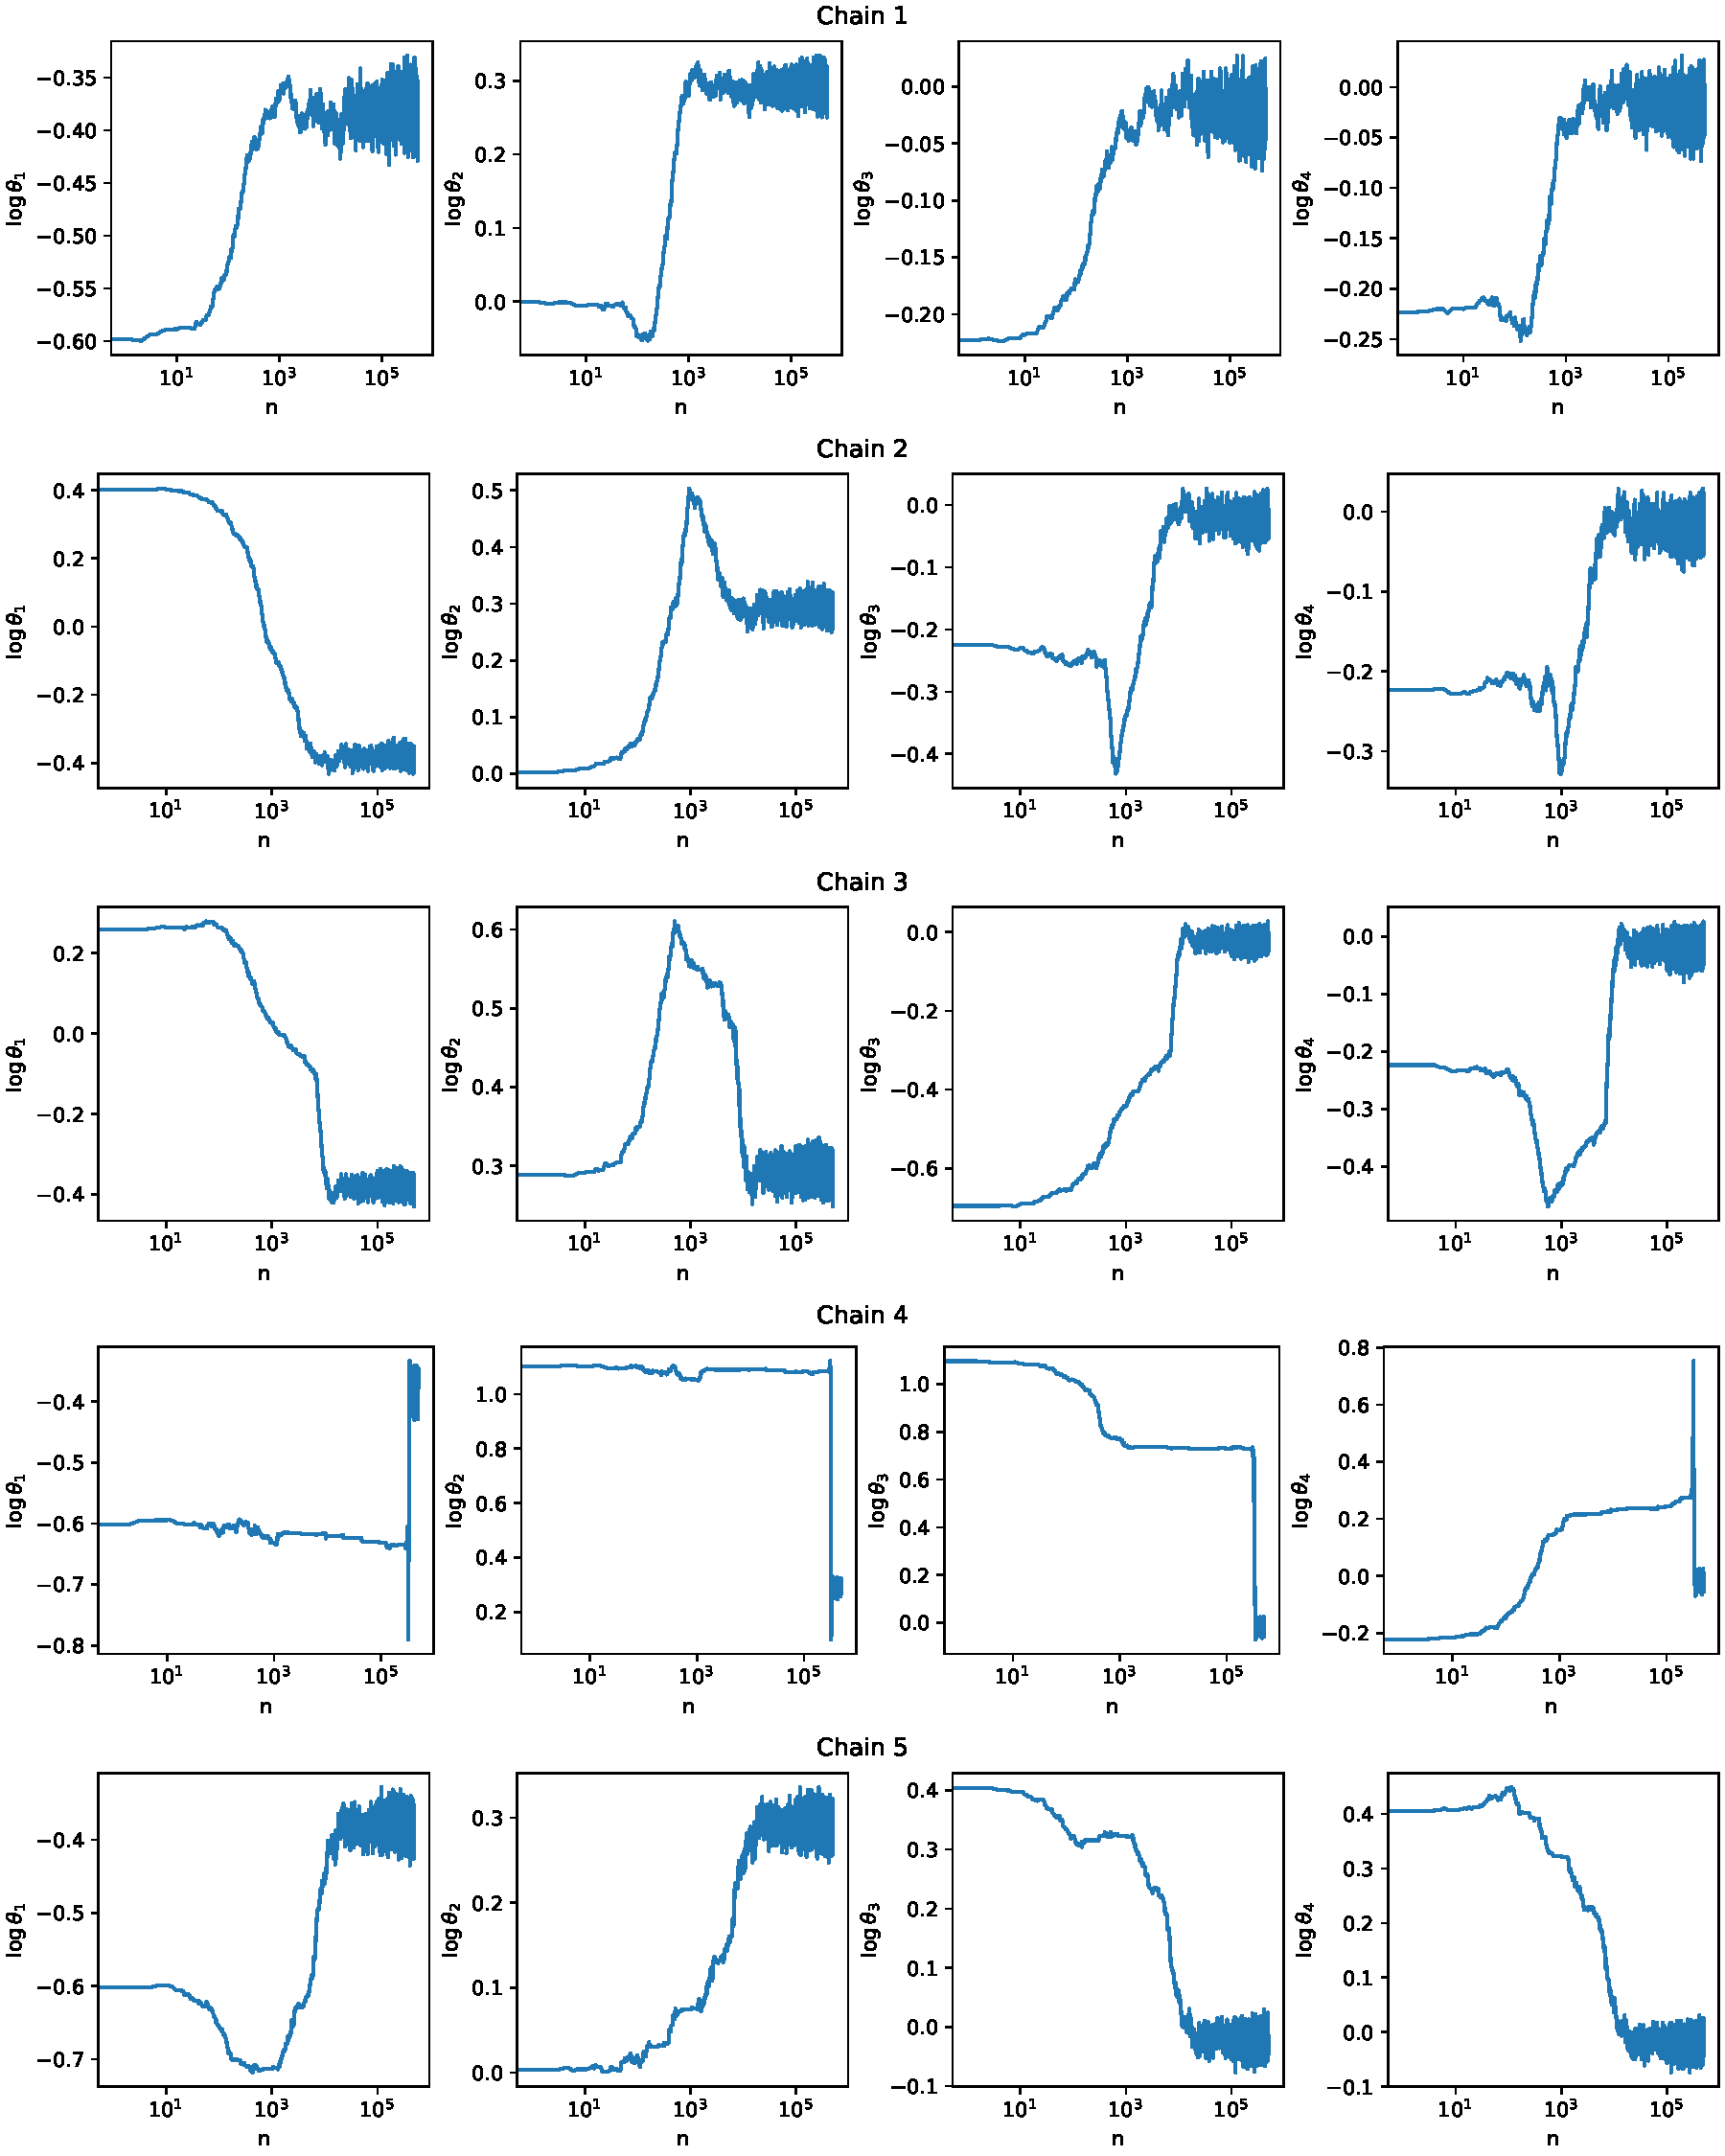
\includegraphics[width=1.0\textwidth]{lotka-volterra-trace-plots.pdf}
}
\caption{Trace plots from the random-walk Metropolis-Hastings algorithm for the Lotka-Volterra inference problem.
\label{fig:lotka-volterra:trace-plots}}
\end{figure}

\begin{figure}[h]
\centering
\makebox[\textwidth][c]{
	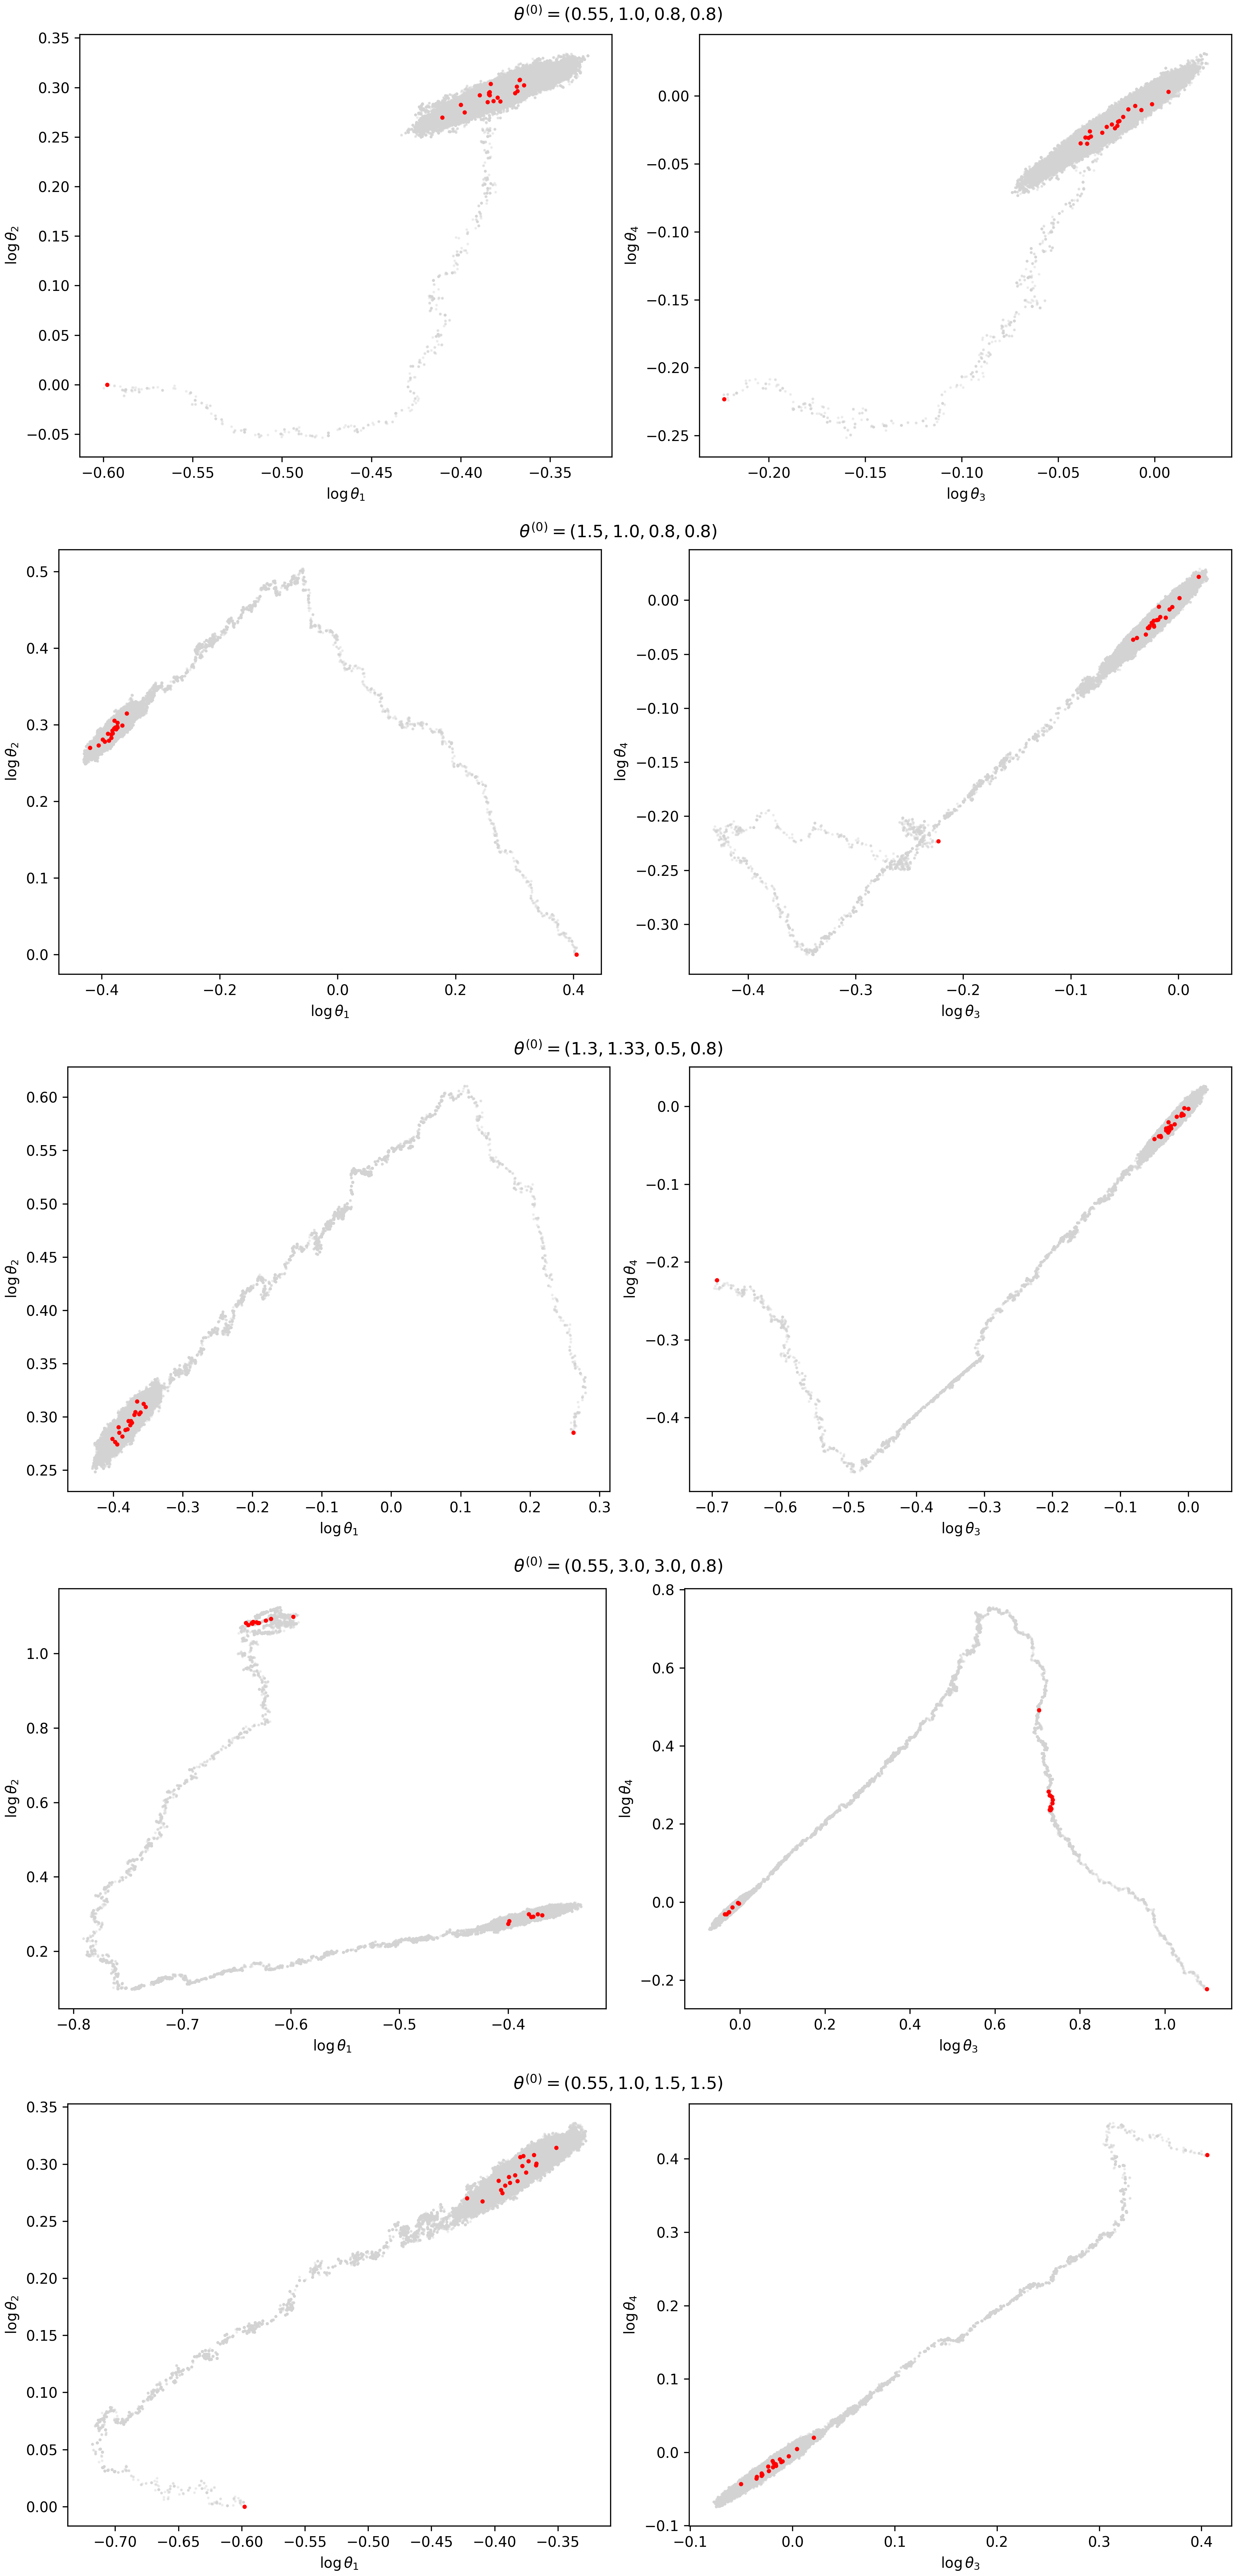
\includegraphics[height=.9\textheight]{lotka-volterra-naive-thinning.png}
}
\caption{Results of na\"ive thinning of the sample from the Lotka-Volterra model.
\label{fig:lotka-volterra:naive:results}}
\end{figure}

\begin{figure}[h]
\centering
\makebox[\textwidth][c]{
	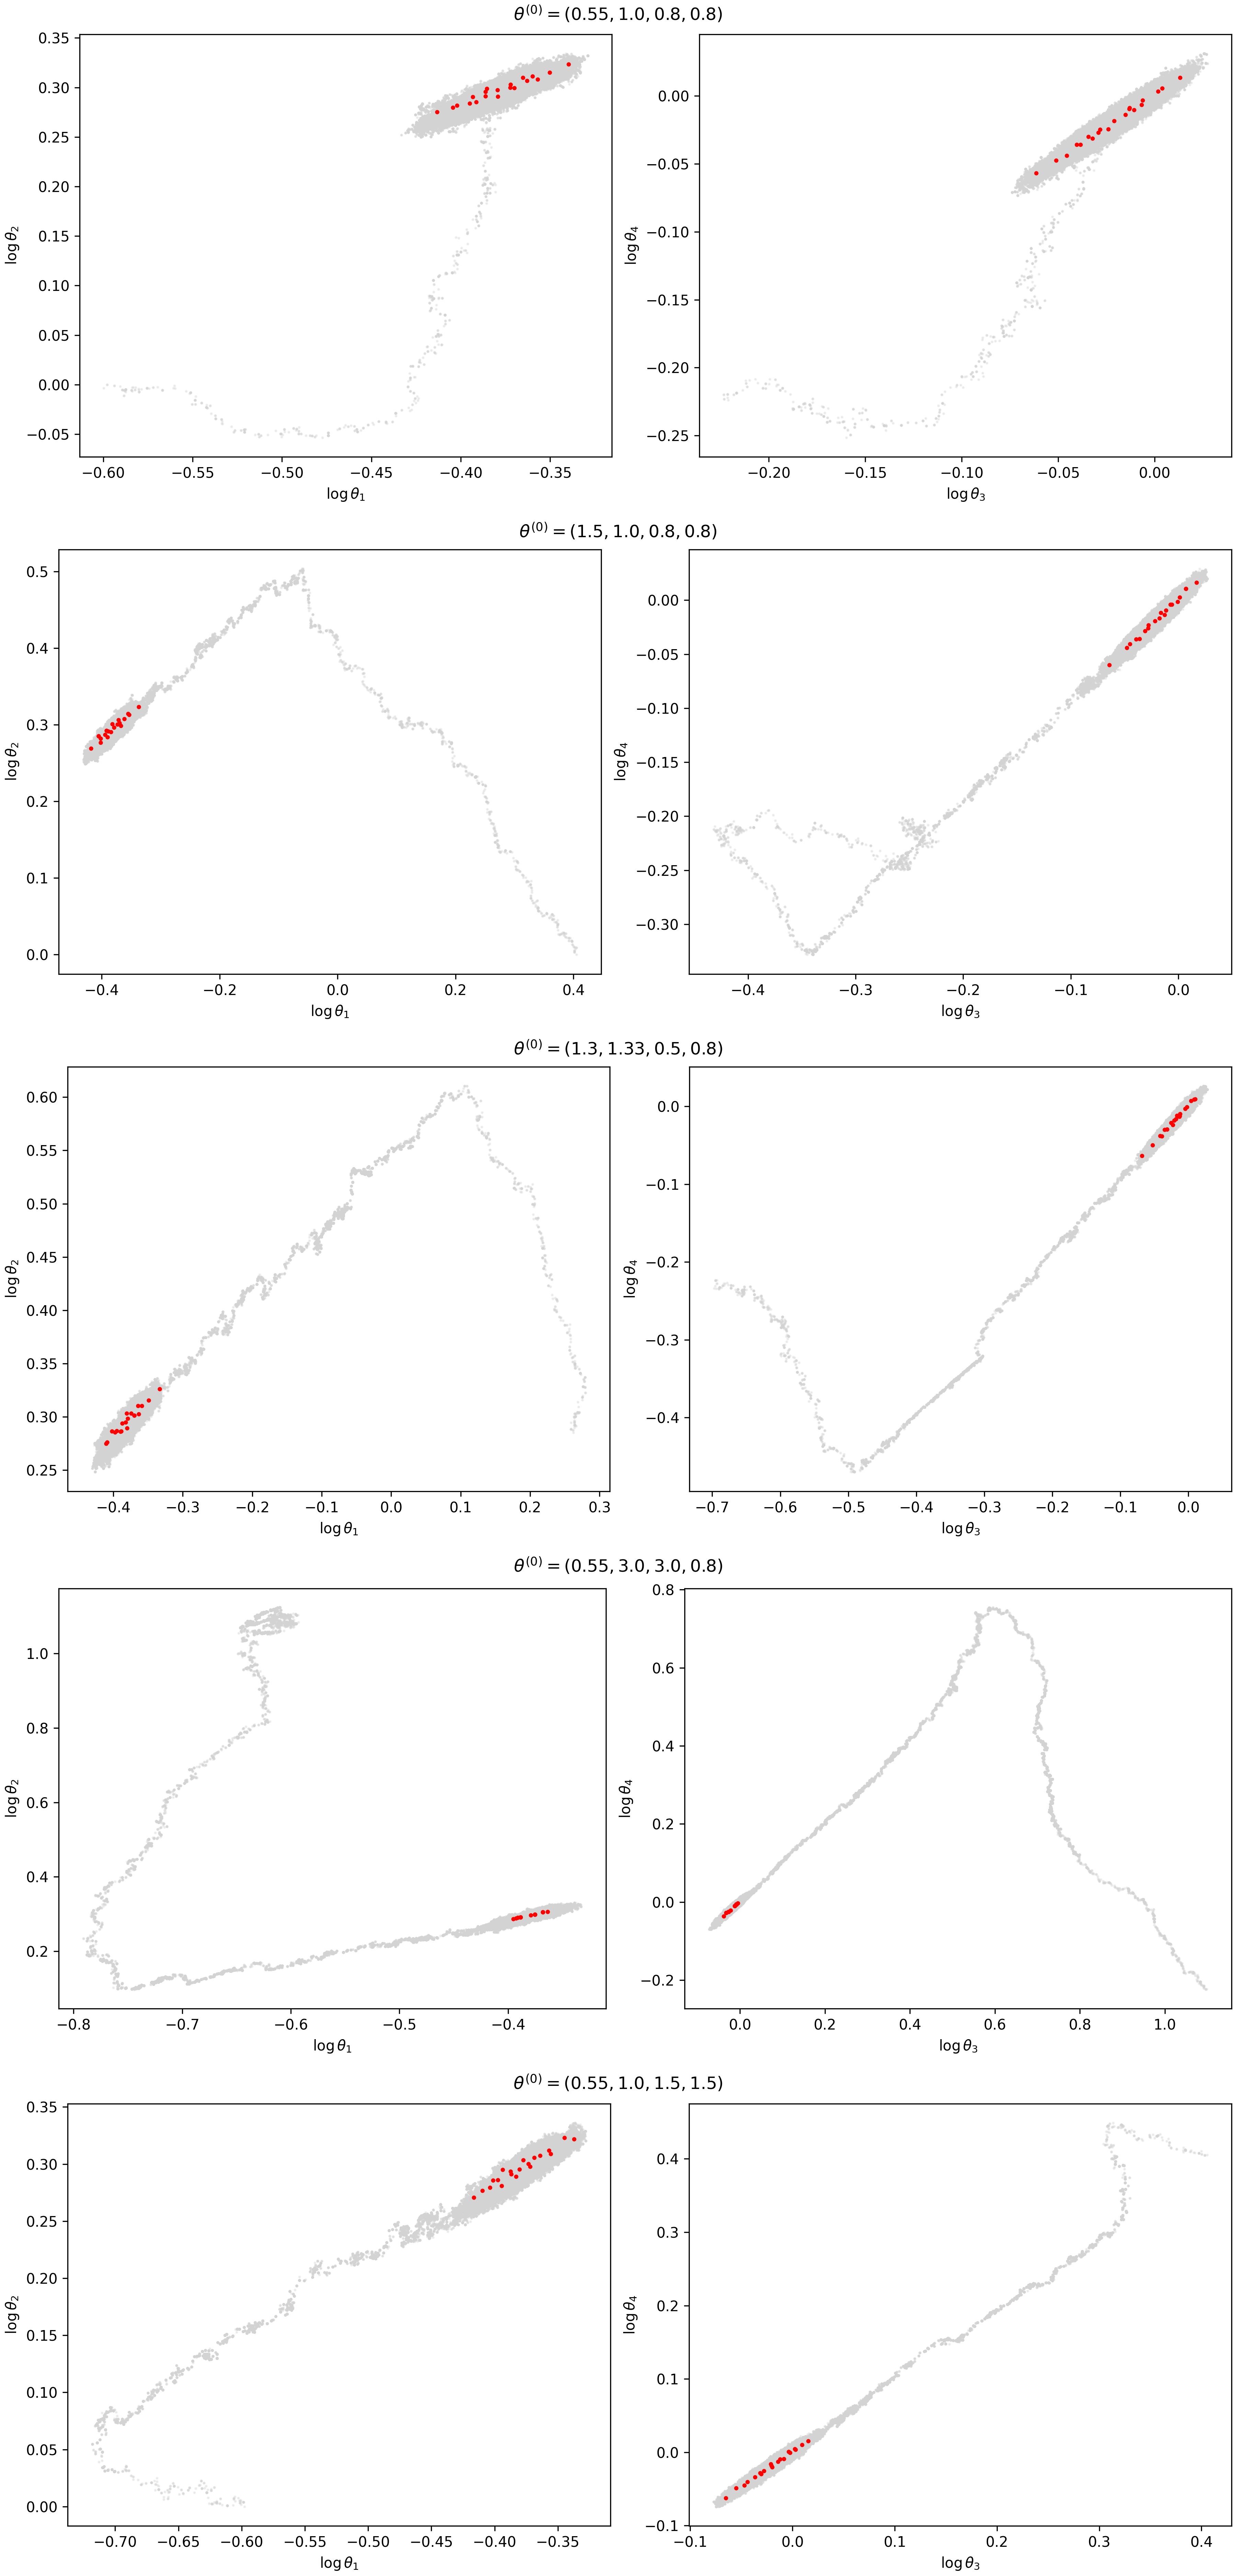
\includegraphics[height=.9\textheight]{lotka-volterra-stein-thinning.png}
}
\caption{The first 20 points selected by the Stein thinning algorithm for each MCMC chain in the Lotka-Volterra inverse problem.
\label{fig:lotka-volterra:stein:results}}
\end{figure}

\end{document}
